
\chapter{Metodologia}
\label{chap:metodologia}

Este capítulo descreve, de forma detalhada, os procedimentos metodológicos
adotados para construção das variáveis, obtenção e tratamento dos dados,
cálculo do \textit{Bitcoin Volatility Risk Premium} (BVRP) e implementação dos
modelos empíricos e de aprendizado de máquina utilizados nesta dissertação.
O processo metodológico foi organizado em quatro etapas principais:

\begin{enumerate}
    \item obtenção e limpeza das séries de preços, volatilidades e índices derivados;
    \item construção da volatilidade implícita (IV30D), da volatilidade realizada (RV30D)
          e do prêmio de risco de volatilidade (BVRP);
    \item definição dos retornos futuros do Bitcoin em diferentes horizontes;
    \item especificação dos modelos estatísticos e de aprendizado de máquina.
\end{enumerate}

\section{Introdução da base de dados}
\label{sec:intro_base}

A base empírica desta dissertação combina informações do mercado à vista de
Bitcoin com medidas de volatilidade implícita do mercado de opções listadas na
Deribit. A partir dessas séries são construídas medidas de volatilidade realizada,
volatilidade implícita em diferentes horizontes e o prêmio de risco de volatilidade
em Bitcoin (BVRP), além de variáveis adicionais como \textit{slopes} da estrutura a termo
e medidas de \textit{skew} extraídas do \textit{smile} de opções.

Os dados são obtidos a partir de três blocos principais:

\begin{enumerate}
    \item histórico do índice DVOL (\textit{Deribit Volatility Index});
    \item superfície de volatilidade implícita de opções de Bitcoin via API pública da Deribit;
    \item preços diários do Bitcoin \textit{spot} em exchanges de alta liquidez.
\end{enumerate}

A presente seção documenta o período da amostra, as fontes de dados, o formato
dos arquivos utilizados, os tratamentos preliminares e a forma de integração entre
as diferentes séries.

\subsection{Visão geral da amostra}

A série de preços \textit{spot} do Bitcoin utilizada no estudo começa em
\textbf{março de 2017} e se estende até \textbf{novembro de 2025}, em frequência diária.
Esse intervalo cobre um número elevado de ciclos de mercado, incluindo fases de
alta acentuada, períodos de realização de lucros, correções abruptas e episódios de
estresse relacionados à liquidação de posições alavancadas em derivativos.

Já o índice DVOL foi oficialmente lançado pela Deribit em
\textbf{31 de março de 2021}, e a série histórica disponibilizada pela própria exchange
tem início nessa data. Assim, para análises que dependem diretamente do DVOL
(como a construção da IV30D a partir do índice), o período efetivo de referência é:

\[
\text{31 de março de 2021 a 30 de novembro de 2025}.
\]

Em contrapartida, para estatísticas descritivas básicas do Bitcoin \textit{spot} e para
algumas análises auxiliares, é possível explorar toda a janela disponível desde 2017.
Ao longo do texto, fica sempre explícito quando uma análise utiliza apenas o
subconjunto de dados pós-2021 (por depender do DVOL) e quando se apoia na
série mais longa de preços do Bitcoin.

\subsection{Fontes de dados e formatos}

\subsubsection*{DVOL (Deribit Volatility Index)}

O primeiro bloco de dados é o histórico diário do índice DVOL, fornecido pela
Deribit em formato CSV. O arquivo contém, para cada dia útil de negociação:

\begin{itemize}
    \item \texttt{timestamp} (data em UTC);
    \item \texttt{open}, \texttt{high}, \texttt{low}, \texttt{close} do índice.
\end{itemize}

O nível do índice é expresso em pontos, equivalentes a uma volatilidade percentual
anualizada. No presente trabalho, utiliza-se o valor de \texttt{close} como medida
diária de volatilidade implícita de 30 dias, definindo-se:

\[
\text{IV30}_t^{\text{(DVOL)}} = \frac{\text{DVOL}_{t,\text{close}}}{100},
\]

em formato decimal.

\subsubsection*{Superfície de volatilidade implícita (API Deribit)}

O segundo bloco é constituído pela superfície de volatilidade implícita das opções
de Bitcoin negociadas na Deribit, obtida por meio de um \textit{pipeline} em Python
que consome a API pública da corretora.

Os principais \textit{endpoints} utilizados são:

\begin{itemize}
    \item \texttt{/public/get\_instruments} — lista todos os contratos de opções
    de Bitcoin ativos, com informações como:
    \begin{itemize}
        \item \texttt{instrument\_name};
        \item \texttt{strike};
        \item \texttt{expiration\_timestamp};
        \item \texttt{option\_type} (call ou put).
    \end{itemize}
    \item \texttt{/public/ticker?instrument\_name=} — retorna, para cada
    contrato, a volatilidade implícita de marcação (\texttt{mark\_iv}), preço de
    marcação e \texttt{delta}, entre outras variáveis.
\end{itemize}

A partir desse conjunto, é possível reconstruir, para datas selecionadas, a superfície
instantânea de IV por \textit{strike} e vencimento, bem como:

\begin{itemize}
    \item construir \textit{smiles} para vencimentos específicos;
    \item calcular \textit{skews} simples (IV média de puts OTM versus calls OTM);
    \item estimar \textit{slopes} da estrutura a termo (por exemplo, IV7D–IV30D,
    IV30D–IV60D).
\end{itemize}

O snapshot estático de instrumentos utilizado no projeto contém centenas de
contratos de opções de Bitcoin, cobrindo múltiplas combinações de \textit{strike} e
vencimento, o que garante granularidade suficiente para análises de curva de
volatilidade e assimetria.

\subsubsection*{Preço \textit{spot} do Bitcoin}

Os preços do Bitcoin \textit{spot} são obtidos a partir de exchanges de alta liquidez
(como Binance e Coinbase), via API ou arquivos históricos padronizados. A base é
convertida para frequência diária, utilizando-se o preço de fechamento próximo
às 23:59 UTC como referência, de modo a manter consistência com o horário de
referência do DVOL e com os dados de opções da Deribit.

A série de preços diários $P_t$ é então transformada em retornos logarítmicos:

\[
r_t = \ln\left(\frac{P_t}{P_{t-1}}\right),
\]

bem como em retornos futuros de diferentes horizontes $h$ dias, que serão
utilizados como variáveis dependentes nos modelos preditivos do Capítulo~\ref{chap:ml}:

\[
r_{t+h} = \ln\left(\frac{P_{t+h}}{P_t}\right),
\quad h \in \{1, 5, 10, 20, 30, 60\}.
\]

\subsection{Tratamento preliminar e limpeza das séries}

Todas as séries passam por um conjunto padronizado de procedimentos de limpeza
e preparação antes da construção das variáveis de volatilidade:

\begin{enumerate}
    \item \textbf{Conversão de datas e timezone}: todas as datas são convertidas
    para o tipo \texttt{datetime} em UTC, garantindo alinhamento temporal
    entre DVOL, superfície de IV e preços \textit{spot}.
    \item \textbf{Ordenação e remoção de duplicatas}: as observações são ordenadas
    cronologicamente e possíveis registros duplicados são removidos.
    \item \textbf{Tratamento de valores ausentes}: dias com ausência de DVOL,
    preços de opções ou preços \textit{spot} são identificados; quando o número
    de faltantes é muito pequeno, as datas são excluídas do painel final para
    evitar imputações arbitrárias.
    \item \textbf{Filtragem de \textit{outliers} evidentes}: são removidos ou
    corrigidos valores claramente distorcidos (por exemplo, resultados implausíveis
    de IV decorrentes de erros pontuais de API).
\end{enumerate}

Ao final desse processo, obtém-se um conjunto diário limpo, pronto para o cálculo
da volatilidade realizada (RV), volatilidade implícita (IV) em múltiplos horizontes,
prêmios de risco de volatilidade (VRP) e demais variáveis explicativas.

\subsection{Integração das bases e painel final}

Após o tratamento individual de cada fonte, as séries são integradas em um painel
diário comum. Em termos gerais, o painel contém, para cada data $t$:

\begin{itemize}
    \item preço \textit{spot} do Bitcoin e retorno diário $r_t$;
    \item DVOL e a correspondente IV30D derivada do índice;
    \item volatilidades realizadas em janelas móveis (RV7D, RV14D, RV30D, RV60D);
    \item volatilidades implícitas extraídas da superfície de opções (IV7D, IV14D,
    IV30D, IV60D), quando disponíveis;
    \item prêmios de risco de volatilidade (VRP7D, VRP14D, VRP30D, VRP60D);
    \item \textit{slopes} da estrutura a termo e medidas de \textit{skew};
    \item retornos futuros $r_{t+h}$ para diferentes horizontes.
\end{itemize}

Como o DVOL só está disponível a partir de 2021, o painel utilizado nas análises
centrais de BVRP e de previsão de retornos corresponde à interseção entre:

\begin{itemize}
    \item a série de preços \textit{spot} (março de 2017 em diante); e
    \item a série oficial do DVOL (a partir de 31 de março de 2021).
\end{itemize}

Esse painel é a base para a análise descritiva detalhada apresentada nas seções
seguintes e para a estimação dos modelos de previsão de retornos desenvolvidos
nos capítulos posteriores.


\section{Descrição do índice DVOL}
\label{sec:dvol}

O índice DVOL (\textit{Deribit Bitcoin Volatility Index}) é a medida de volatilidade
implícita de 30 dias desenvolvida pela Deribit e publicada diariamente desde
31 de março de 2021. O objetivo do índice é fornecer uma estimativa sintética e
padronizada da volatilidade implícita de curto prazo do Bitcoin, desempenhando um
papel análogo ao do VIX para o mercado acionário americano.

O DVOL é amplamente utilizado como referência por participantes institucionais,
gestores quantitativos e \textit{market makers}, servindo como uma aproximação da
volatilidade implícita ATM (at-the-money) para 30 dias. Nesta dissertação, o índice
constitui a fonte primária para a volatilidade implícita de 30 dias (\textbf{IV30D})
utilizada na construção do prêmio de risco de volatilidade do Bitcoin (BVRP).

\subsection{Metodologia geral de cálculo}

Embora a Deribit não divulgue integralmente a fórmula proprietária do DVOL,
o método segue a lógica fundamental empregada na construção do VIX: integrar os
preços de opções OTM de diferentes strikes para uma maturidade alvo de 30 dias,
de modo a estimar uma variância neutra ao risco agregada. Em termos conceituais,
o índice pode ser interpretado como:

\[
\text{DVOL}_t = 100 \times \sqrt{ \sigma^2_{t}(30\,\text{dias}) },
\]

onde $\sigma^2_{t}(30\,\text{dias})$ representa a variância implícita de 30 dias
extraída da superfície de opções.

De forma análoga à formulação do VIX, uma representação genérica pode ser
escrita como:

\[
\sigma^2_{t}(T) = 
\frac{2 e^{rT}}{T}
\sum_{i \in \mathcal{K}} 
\frac{\Delta K_i}{K_i^2} Q(K_i, T)
-
\frac{1}{T}
\left( \frac{F}{K_{\text{ATM}}} - 1 \right)^2,
\]

em que:

\begin{itemize}
    \item $T$ é o prazo de 30 dias expresso em anos;
    \item $K_i$ são os strikes discretizados;
    \item $\Delta K_i$ é o espaçamento entre strikes adjacentes;
    \item $Q(K_i, T)$ é o preço da opção OTM (call ou put, conforme o strike);
    \item $F$ é o preço a termo do Bitcoin para o vencimento alvo;
    \item $K_{\text{ATM}}$ é o strike mais próximo do preço a termo.
\end{itemize}

Essa expressão é ilustrativa; a Deribit utiliza ajustes proprietários, incluindo pesos,
regiões específicas de strikes e suavizações para lidar com irregularidades na
superfície. Ainda assim, a essência permanece: o DVOL é uma medida de volatilidade
implícita agregada para o horizonte fixo de 30 dias.

\subsection{Conversão e uso no presente estudo}

Para fins desta dissertação, o nível diário do DVOL é convertido para formato
decimal, resultando na volatilidade implícita ATM de 30 dias:

\[
\text{IV30D}_t = \frac{\text{DVOL}_{t,\text{close}}}{100}.
\]

Esta é a medida de volatilidade implícita utilizada para construir o prêmio de
risco de volatilidade de 30 dias:

\[
\text{VRP30D}_t = \text{IV30D}_t - \text{RV30D}_t,
\]

onde $\text{RV30D}_t$ é a volatilidade realizada em 30 dias, calculada a partir dos
retornos logarítmicos do Bitcoin.

\subsection{Por que utilizar o DVOL?}

\begin{enumerate}
    \item \textbf{Liquidez elevada}: o mercado de opções de Bitcoin da Deribit é o mais
    líquido globalmente, concentrando a maioria das negociações institucionais.
    \item \textbf{Medida consolidada}: o DVOL é uma métrica agregada e menos ruidosa
    do que extrair IV30 diretamente de um strike específico.
    \item \textbf{Comparabilidade}: sua interpretação é consistente com índices de
    volatilidade tradicionais, facilitando análises intertemporais e entre classes
    de ativos.
    \item \textbf{Estabilidade}: por ser baseado em integração de vários strikes, o
    índice é menos sujeito a distorções microestruturais pontuais.
\end{enumerate}

\subsection{Limitações do DVOL}

Apesar das vantagens, algumas limitações precisam ser reconhecidas:

\begin{itemize}
    \item \textbf{Disponibilidade histórica limitada}: o DVOL só existe oficialmente
    a partir de 2021, restringindo a janela de estudos envolvendo o prêmio de
    risco de volatilidade.
    \item \textbf{Cálculo proprietário}: detalhes completos da fórmula não são
    divulgados, o que limita reprodutibilidade total.
    \item \textbf{Foco ATM}: o DVOL representa essencialmente IV ATM; informações
    importantes de assimetria (\textit{skew}) e estrutura a termo dependem da
    superfície e não são capturadas pelo índice.
    \item \textbf{Sensibilidade a horários}: discrepâncias entre horários de coleta
    podem introduzir ruídos se não houver padronização (tratada nesta dissertação
    via sincronização em UTC).
\end{itemize}

\subsection{Integração com a superfície de IV}

Embora o DVOL seja utilizado como proxy principal para IV30D, esta dissertação
também utiliza informações da superfície de volatilidade implícita obtida pela API da
Deribit para:

\begin{itemize}
    \item calcular \textit{skew} (puts OTM vs. calls OTM);
    \item estimar \textit{slopes} da estrutura a termo (IV7D–IV30D, IV30D–IV60D);
    \item validar a consistência da IV30 derivada do DVOL com a IV30 interpolada
    diretamente da superfície.
\end{itemize}

Essa integração permite investigar nuances da estrutura de volatilidade que não
estão presentes no DVOL, além de fornecer medidas adicionais para os modelos
preditivos do Capítulo~\ref{chap:ml}.

\section{Retornos futuros}

Para avaliar o potencial preditivo do BVRP, foram construídos retornos futuros
em três horizontes:

\begin{align*}
\text{ret\_fut\_1d} &= \ln(P_{t+1}) - \ln(P_t), \\
\text{ret\_fut\_5d} &= \ln(P_{t+5}) - \ln(P_t), \\
\text{ret\_fut\_20d} &= \ln(P_{t+20}) - \ln(P_t).
\end{align*}

Esses horizontes capturam diferentes dinâmicas:

\begin{itemize}
    \item \textbf{1 dia}: reações imediatas a condições de mercado;
    \item \textbf{5 dias}: janela semanal típica do mercado cripto;
    \item \textbf{20 dias}: horizonte mensal, que suaviza movimentos de curto prazo.
\end{itemize}

\section{Descrição do conjunto final de variáveis}

A Tabela~\ref{tab:estatisticas_cap4} resume as variáveis empregadas nos
modelos:

\begin{itemize}
    \item volatilidades: IV30D, RV30D, BVRP;
    \item retornos futuros: 1D, 5D e 20D;
    \item preço spot do Bitcoin (nível e retornos passados);
    \item medidas de tendência (retornos acumulados);
    \item volatilidades realizadas curtas (RV7D, RV14D);
    \item defasagens das principais variáveis (lags).
\end{itemize}

O conjunto final combina informações contemporâneas e defasadas, permitindo que
os modelos capturem estruturas temporais e não linearidades.

\section{Modelos estatísticos}

A análise inicial emprega ferramentas de estatística clássica:

\begin{itemize}
    \item gráficos de dispersão entre BVRP e retornos futuros;
    \item correlações de Pearson;
    \item regressões lineares simples da forma:
\[
ret\_fut_{h,t} = \alpha + \beta \cdot BVRP_t,
\]
\end{itemize}

que fornecem evidências preliminares sobre a relação entre BVRP e retornos.

\section{Modelos de aprendizado de máquina}

Para capturar potenciais não-linearidades e interações entre variáveis, foram
implementados dois algoritmos amplamente utilizados em aplicações financeiras:
Random Forest e XGBoost.

\subsection{Random Forest}

O Random Forest \citep{breiman2001randomforest} utiliza uma abordagem de
\textit{bagging}, combinando múltiplas árvores treinadas em amostras bootstrap.
Os principais hiperparâmetros utilizados foram:

\begin{itemize}
    \item 500 árvores;
    \item amostragem bootstrap padrão;
    \item profundidade máxima não restrita;
    \item seleção aleatória de subconjuntos de variáveis por nó.
\end{itemize}

Esse método é robusto a ruído, captura relações não lineares e interações entre
variáveis, e é pouco sensível a escala ou transformações monotônicas.

\subsection{XGBoost}

O XGBoost \citep{chen2016xgboost} emprega \textit{gradient boosting} com
regularização explícita, construindo árvores de forma sequencial. A cada etapa,
uma nova árvore busca corrigir os erros residuais da árvore anterior. Os
principais hiperparâmetros utilizados foram:

\begin{itemize}
    \item 300 árvores;
    \item taxa de aprendizado $\eta = 0.05$;
    \item profundidade máxima igual a 4;
    \item regularização L2.
\end{itemize}

O XGBoost é particularmente eficiente na detecção de padrões fracos de
previsão, sendo uma das abordagens mais bem-sucedidas em competições e
aplicações práticas em finanças.

\section{Validação dos modelos}

A avaliação dos modelos foi realizada por meio de:

\begin{itemize}
    \item separação da amostra em 70\% treino e 30\% teste;
    \item métricas de erro: MSE, MAE e correlação entre valores previstos e realizados;
    \item inspeção gráfica dos resíduos e das previsões.
\end{itemize}

Essa abordagem permite avaliar tanto o desempenho preditivo quanto a aderência
estrutural dos modelos.

\section{Síntese do capítulo}

Este capítulo detalhou os procedimentos metodológicos utilizados na construção
das variáveis, no cálculo do BVRP, na definição dos retornos futuros e na
implementação dos modelos estatísticos e de aprendizado de máquina. Esses
elementos formam a base para a análise empírica apresentada no
Capítulo~\ref{chap:resultados}, que discute as principais evidências obtidas a
partir dos dados.

\chapter{Resultados Iniciais e Estatísticas Descritivas}
\label{chap:resultados_iniciais}

Este capítulo apresenta os primeiros resultados empíricos relacionados ao
comportamento da volatilidade implícita (IV30D), da volatilidade realizada
(RV30D) e do prêmio de risco de volatilidade em Bitcoin (BVRP).
O objetivo é fornecer uma visão descritiva inicial das séries, destacando
padrões estatísticos, tendências gerais e possíveis indícios preliminares de
relação entre o BVRP e retornos futuros do Bitcoin. Essas evidências funcionam
como base para as análises aprofundadas desenvolvidas nos capítulos seguintes.

\section{Comportamento geral da volatilidade}

O mercado de Bitcoin é amplamente reconhecido por sua elevada volatilidade,
característica que se manifesta de forma consistente tanto na volatilidade
realizada quanto na volatilidade implícita. Em condições típicas de mercado, a
volatilidade anualizada tende a oscilar entre 40\% e 80\%, podendo ultrapassar
100\% durante episódios de estresse, liquidações alavancadas ou choques
idiossincráticos.

De maneira geral:

\begin{itemize}
    \item a \textbf{IV30D} apresenta comportamento mais suave e reage de forma gradual
          a eventos, refletindo a natureza agregada das expectativas do mercado;
    \item a \textbf{RV30D} é mais ruidosa e exibe saltos abruptos, devido à
          microestrutura do mercado de Bitcoin e à ocorrência de movimentos
          repentinos de preço;
    \item o \textbf{BVRP}, calculado como a diferença entre IV30D e RV30D,
          resume de modo sintético o prêmio pago pelo mercado pela incerteza
          futura.
\end{itemize}

Essas características tornam o estudo do BVRP particularmente relevante em
mercados com volatilidade estruturalmente elevada, como o de criptoativos.

\section{Estatísticas descritivas básicas}
\label{sec:estatisticas_basicas}

A Tabela~\ref{tab:estatisticas_cap4} apresenta as estatísticas descritivas
(média, desvio-padrão, mínimos e máximos) das principais variáveis empregadas:
volatilidade implícita (IV30D), volatilidade realizada (RV30D), prêmio de risco
de volatilidade (BVRP) e retornos futuros do Bitcoin em horizontes de 1, 5 e
20 dias.

\input{tabela_cap4_estatisticas_completas}

Os resultados mostram que a IV30D mantém média superior à RV30D, implicando um
BVRP positivo no período analisado, embora com dispersão considerável. Essa
dispersão está alinhada com a natureza altamente volátil do Bitcoin, cujos
choques de preço podem gerar episódios de divergência acentuada entre IV e RV.
Os retornos futuros exibem assimetria e caudas pronunciadas, destacando a
presença de eventos extremos — tanto de queda quanto de valorização — no
horizonte considerado. Esses achados estão em conformidade com a literatura que
documenta prêmios de volatilidade positivos em mercados de opções e a presença
de distribuições com caudas pesadas em criptoativos.

\section{Primeira visualização das séries}

A inspeção inicial das séries indica que:

\begin{itemize}
    \item períodos de aumento acentuado na IV30D coincidem com momentos de maior
          incerteza e elevação na demanda por proteção;
    \item a RV30D exibe maior variabilidade e maior frequência de \textit{outliers},
          frequentemente associados a movimentos bruscos de preço;
    \item o BVRP oscila entre valores positivos e negativos, com predominância
          de valores positivos, sugerindo que o mercado tende a precificar a
          volatilidade futura acima da volatilidade realizada.
\end{itemize}

A dinâmica temporal detalhada dessas séries será explorada no
Capítulo~\ref{chap:analise_empirica}, onde são analisados períodos específicos,
episódios de estresse e regimes distintos de volatilidade.

\section{Inspeção inicial da relação entre BVRP e retornos}

A análise exploratória preliminar sugere que:

\begin{itemize}
    \item a correlação entre BVRP e retornos de curtíssimo prazo (1 dia) é
          bastante baixa, indicando que o BVRP tem impacto limitado em janelas
          muito curtas;
    \item a relação se intensifica ligeiramente em retornos de 5 dias;
    \item a associação torna-se mais evidente no horizonte de 20 dias, embora
          ainda moderada.
\end{itemize}

Esses padrões são consistentes com estudos que sugerem que os efeitos do VRP
tendem a emergir em horizontes mais longos, quando a volatilidade realizada tem
maior probabilidade de convergir para suas expectativas implícitas.

\section{Limitações desta análise inicial}

Cabe destacar algumas limitações desta etapa descritiva:

\begin{itemize}
    \item a análise é exclusivamente exploratória, não permitindo inferências
          causais entre o BVRP e os retornos do Bitcoin;
    \item o BVRP é sensível a discrepâncias pontuais entre IV e RV, que podem
          distorcer relações em janelas curtas;
    \item retornos futuros do Bitcoin são influenciados por múltiplos fatores
          não capturados nesta inspeção inicial.
\end{itemize}

Essas limitações serão abordadas por meio de modelos estatísticos e de
aprendizado de máquina nos capítulos subsequentes.

\section{Síntese do capítulo}

Este capítulo apresentou uma visão introdutória sobre o comportamento da
volatilidade implícita, da volatilidade realizada e do BVRP em Bitcoin. Os
resultados iniciais evidenciam um mercado estruturalmente volátil, com eventos
extremos que influenciam de maneira assimétrica as medidas de volatilidade e os
retornos futuros.

A análise detalhada, incluindo gráficos completos, identificação de regimes e
avaliação da capacidade preditiva do BVRP, será desenvolvida no
Capítulo~\ref{chap:analise_empirica}.

\chapter{Análise Empírica do Prêmio de Risco de Volatilidade em Bitcoin (BVRP)}
\label{chap:analise_empirica}

Este capítulo aprofunda a investigação empírica do \textit{Bitcoin Volatility
Risk Premium} (BVRP), examinando suas propriedades estatísticas, sua evolução
temporal, seus regimes, sua distribuição e sua relação visual com retornos
futuros do Bitcoin. Os resultados apresentados aqui complementam e aprofundam as
estatísticas descritivas discutidas no Capítulo~\ref{chap:resultados_iniciais}.

\section{Evolução temporal do VRP}

A Figura~\ref{fig:vrp_timeseries} apresenta a trajetória conjunta da
volatilidade implícita a 30 dias (IV30D), da volatilidade realizada (RV30D) e do
BVRP ao longo da amostra completa.

\begin{figure}[H]
    \centering
    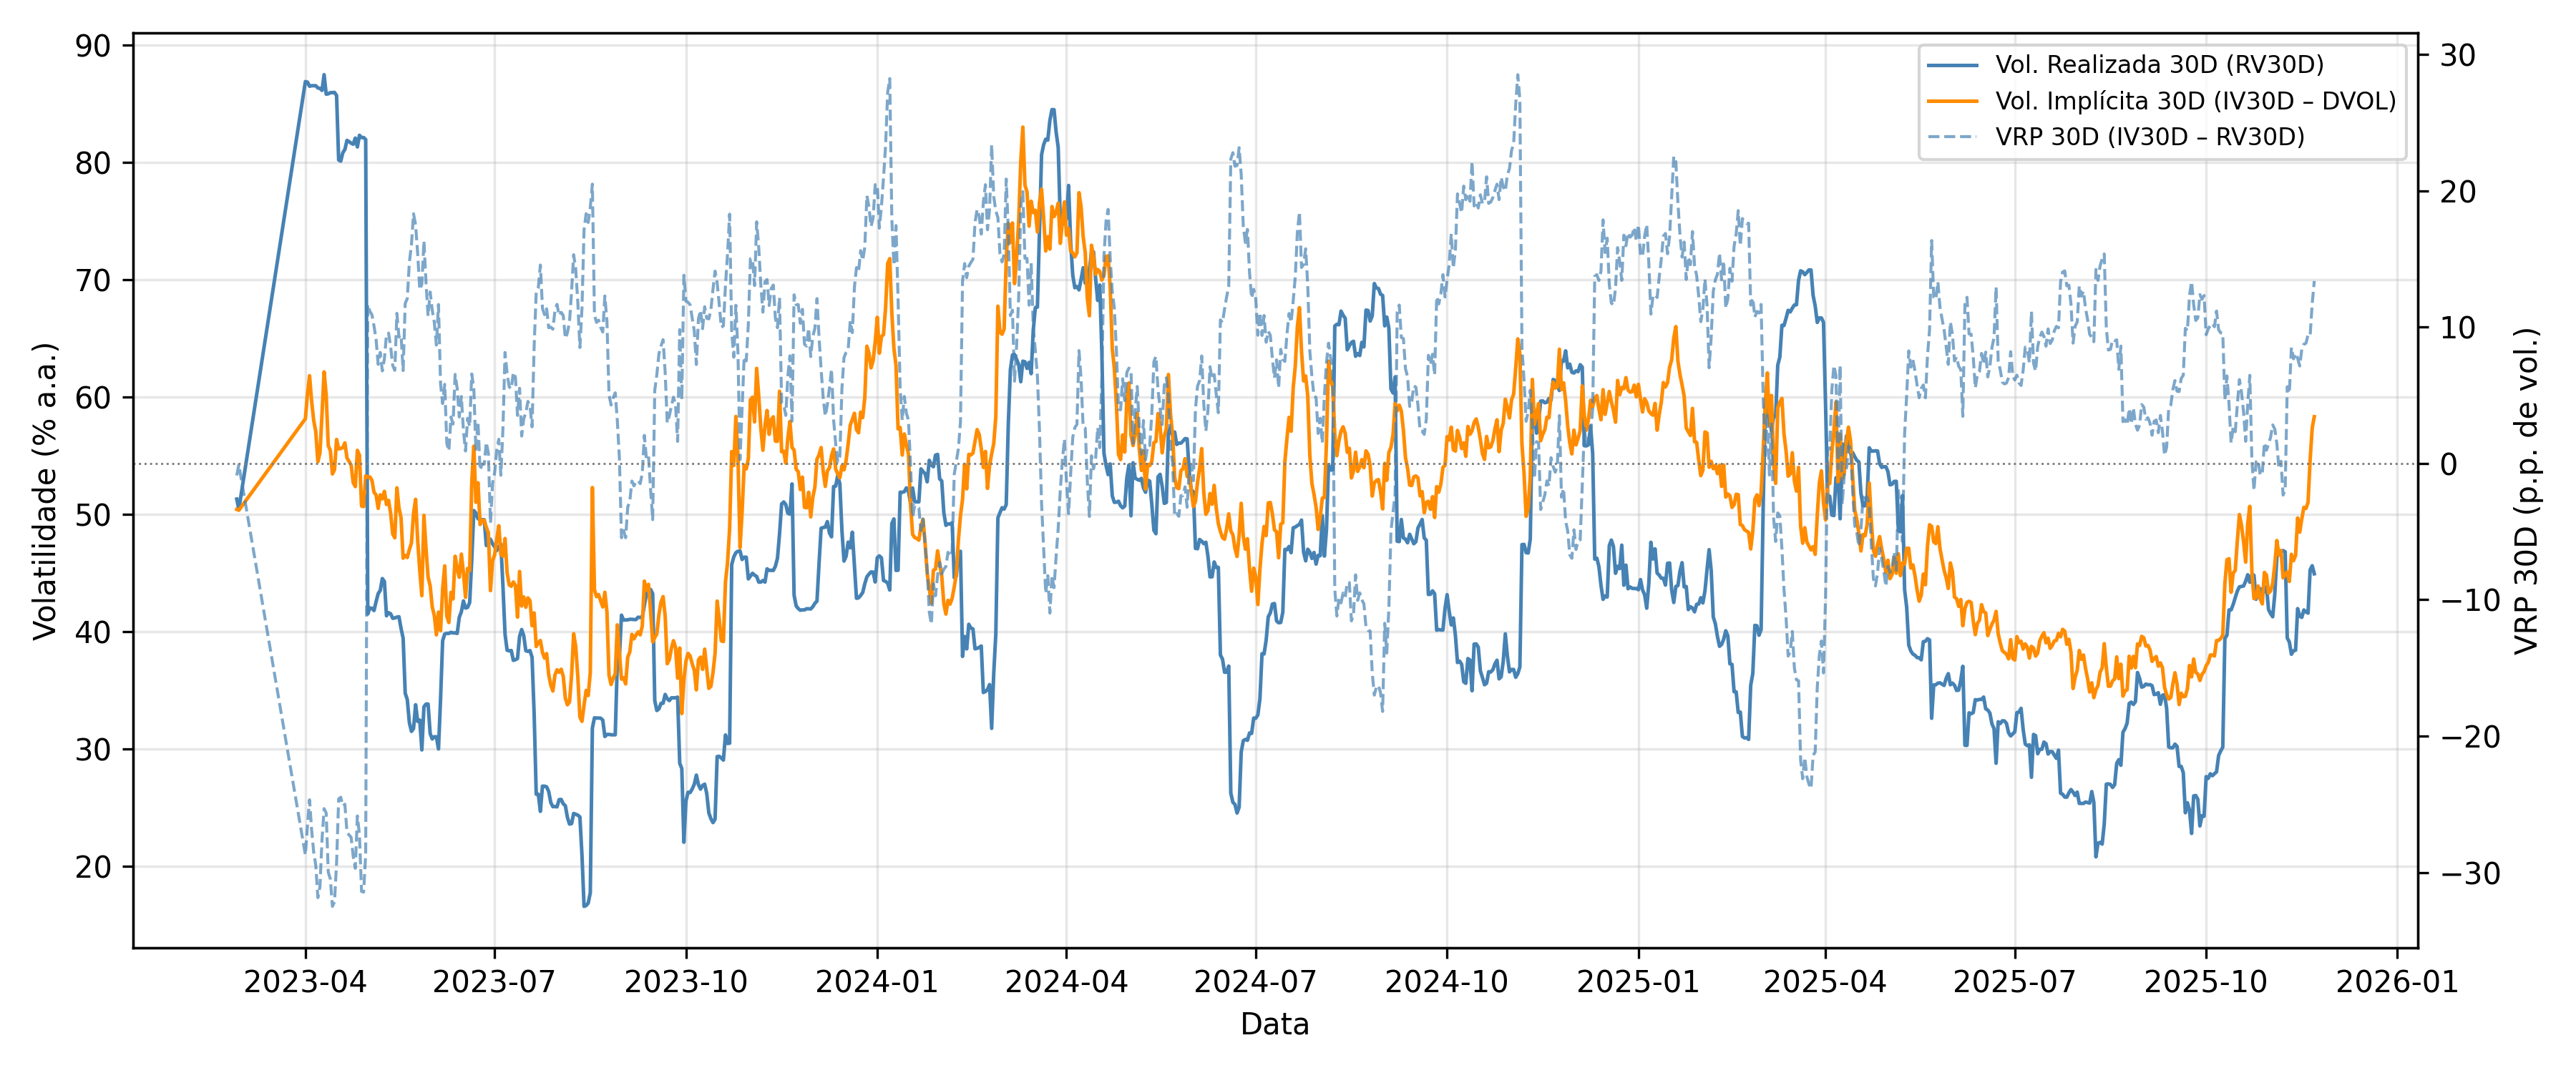
\includegraphics[width=\textwidth]{figs/vrp_timeseries.png}
    \caption{Evolução temporal da IV30D, RV30D e do BVRP.}
    \label{fig:vrp_timeseries}
\end{figure}

A série revela alguns padrões importantes:

\begin{itemize}
    \item a IV30D frequentemente se mantém acima da RV30D, sugerindo um prêmio de
          proteção estruturalmente positivo;
    \item episódios de VRP negativo ocorrem tipicamente após movimentos bruscos
          do preço do Bitcoin, quando a volatilidade realizada salta de forma
          acentuada;
    \item o BVRP exibe clusters de regimes, com períodos prolongados de
          complacência (VRP elevado) seguidos de fases de estresse (VRP próximo
          de zero ou negativo).
\end{itemize}

Esse comportamento é consistente com a literatura que documenta regimes de
volatilidade e saltos associados a liquidações e eventos idiossincráticos no
mercado de criptoativos.

\section{Distribuição do BVRP}

A Figura~\ref{fig:vrp_histogram_kde} exibe o histograma da distribuição empírica
do BVRP, acompanhado de uma densidade suavizada (KDE).

\begin{figure}[H]
    \centering
    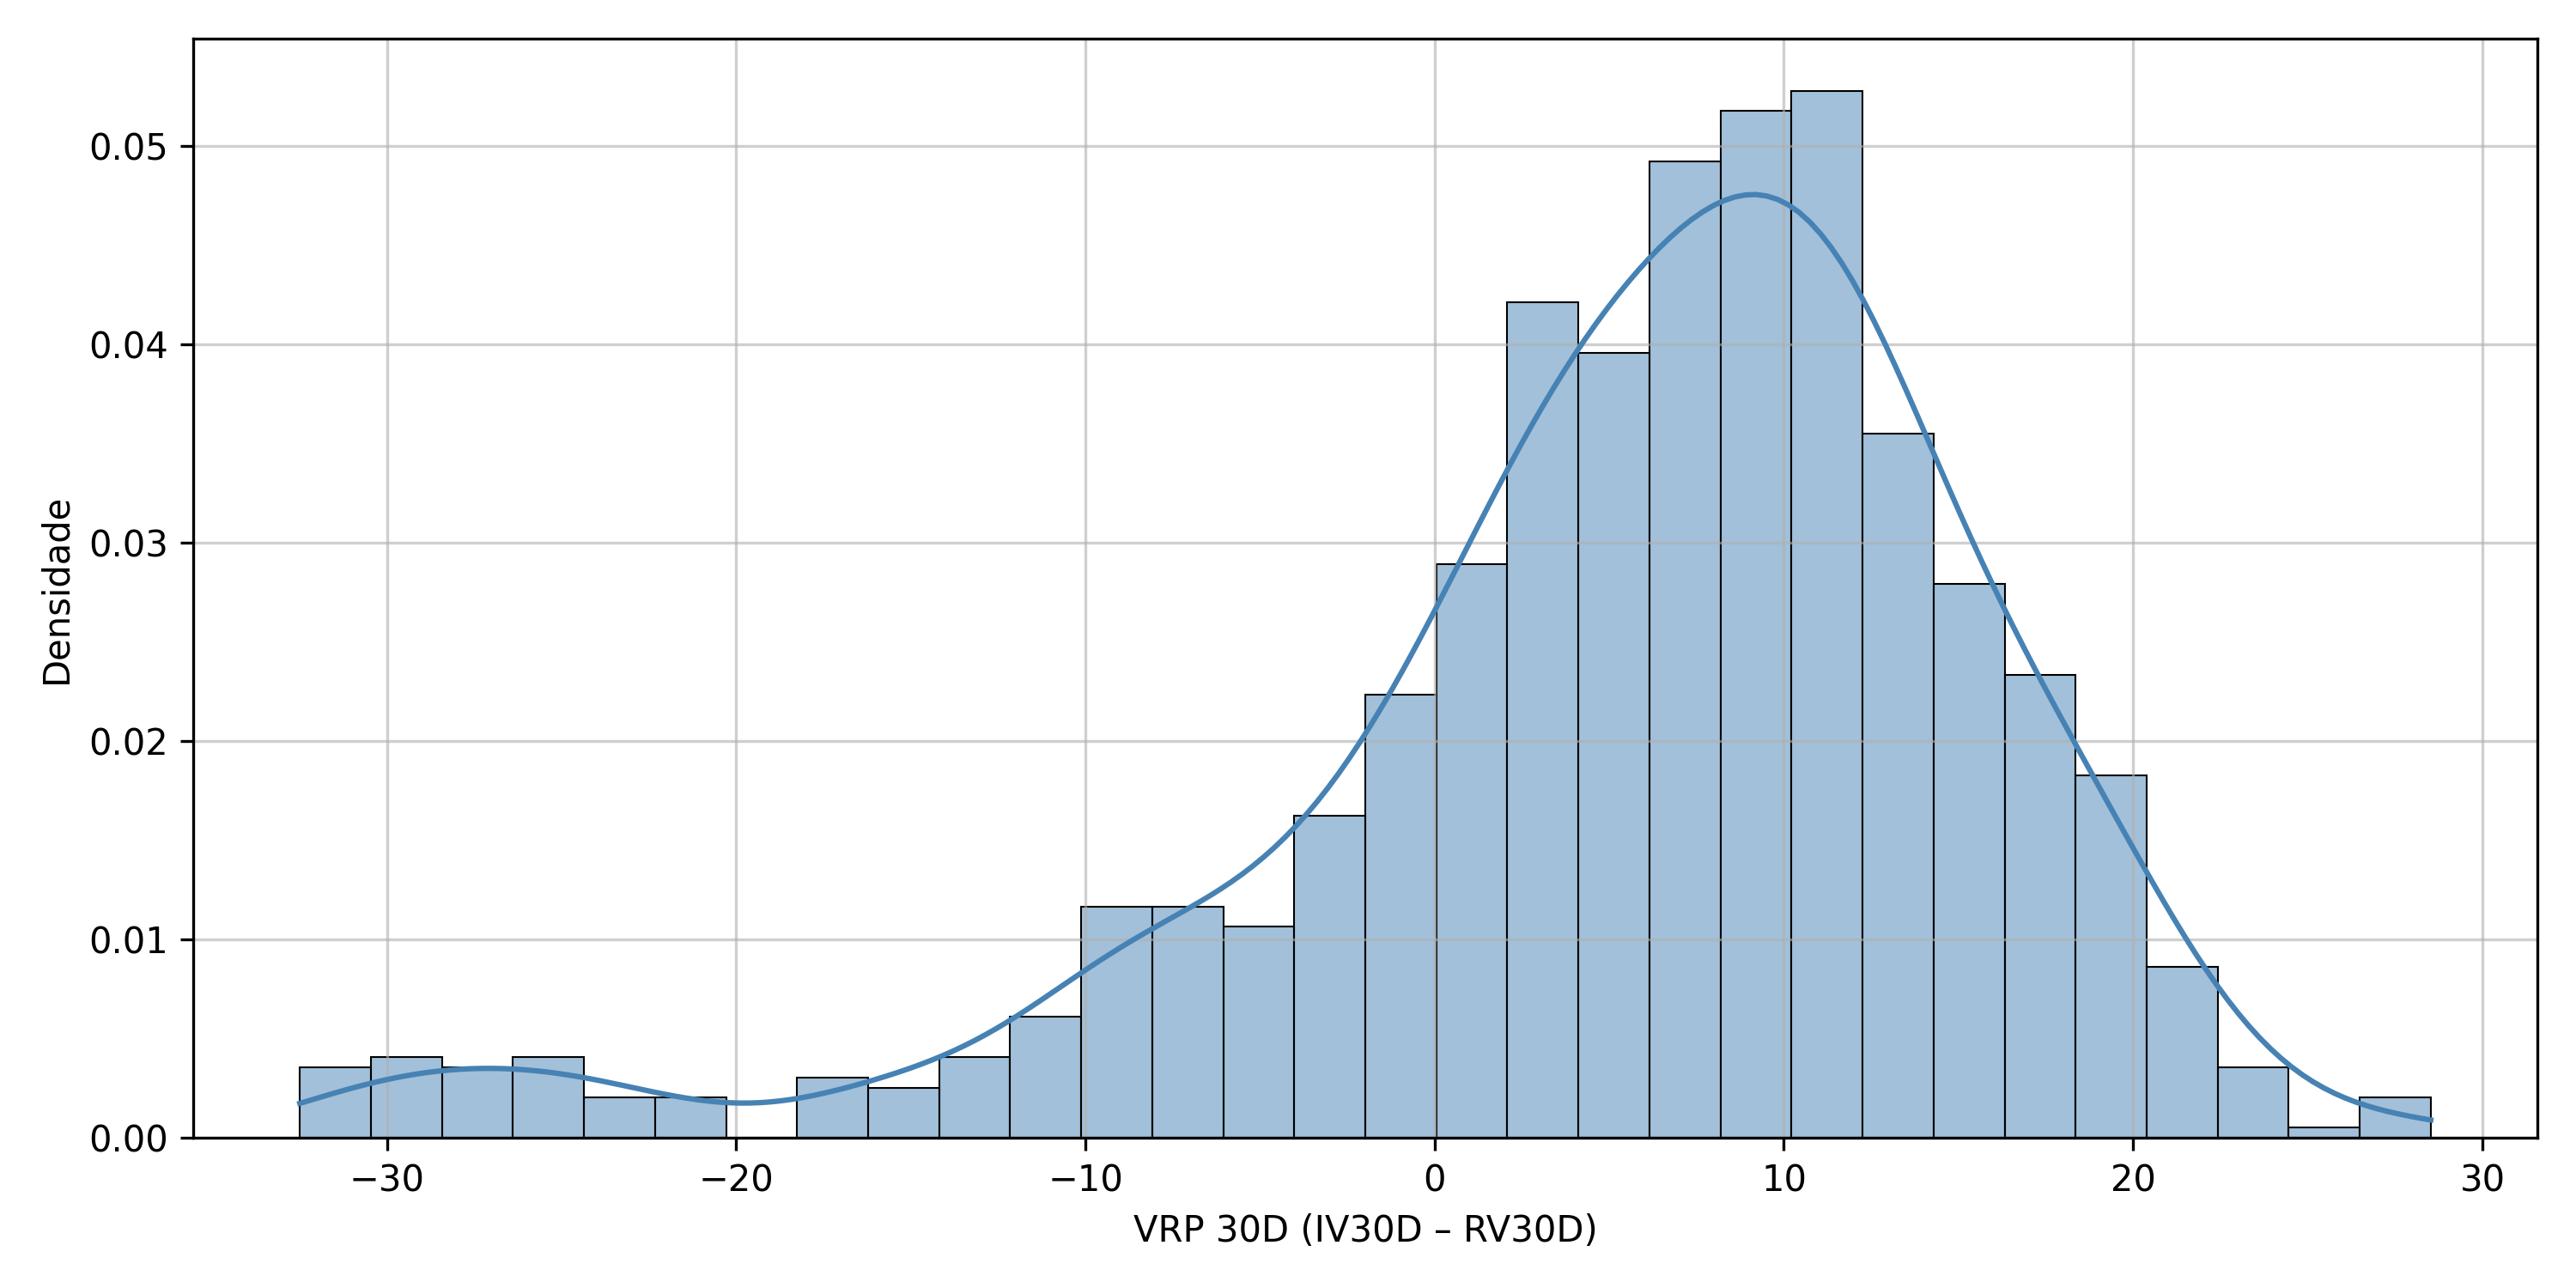
\includegraphics[width=0.92\textwidth]{figs/vrp_histogram_kde.png}
    \caption{Distribuição empírica do VRP (histograma + KDE).}
    \label{fig:vrp_histogram_kde}
\end{figure}

A distribuição apresenta características marcantes:

\begin{itemize}
    \item predominância de valores positivos, refletindo o padrão estrutural de
          demanda por proteção;
    \item cauda inferior alongada, atribuída a períodos em que a RV30D supera de
          forma abrupta a IV30D, geralmente em eventos extremos;
    \item presença de picos moderados de VRP elevado, indicativos de períodos de
          complacência.
\end{itemize}

Essas características são decisivas para avaliar o potencial preditivo do VRP e
para justificar técnicas não lineares na etapa de modelagem.

\section{BVRP por período e por ano}

O boxplot geral do BVRP, apresentado na Figura~\ref{fig:vrp_boxplot}, resume a
variabilidade da série ao longo do período analisado.

\begin{figure}[H]
    \centering
    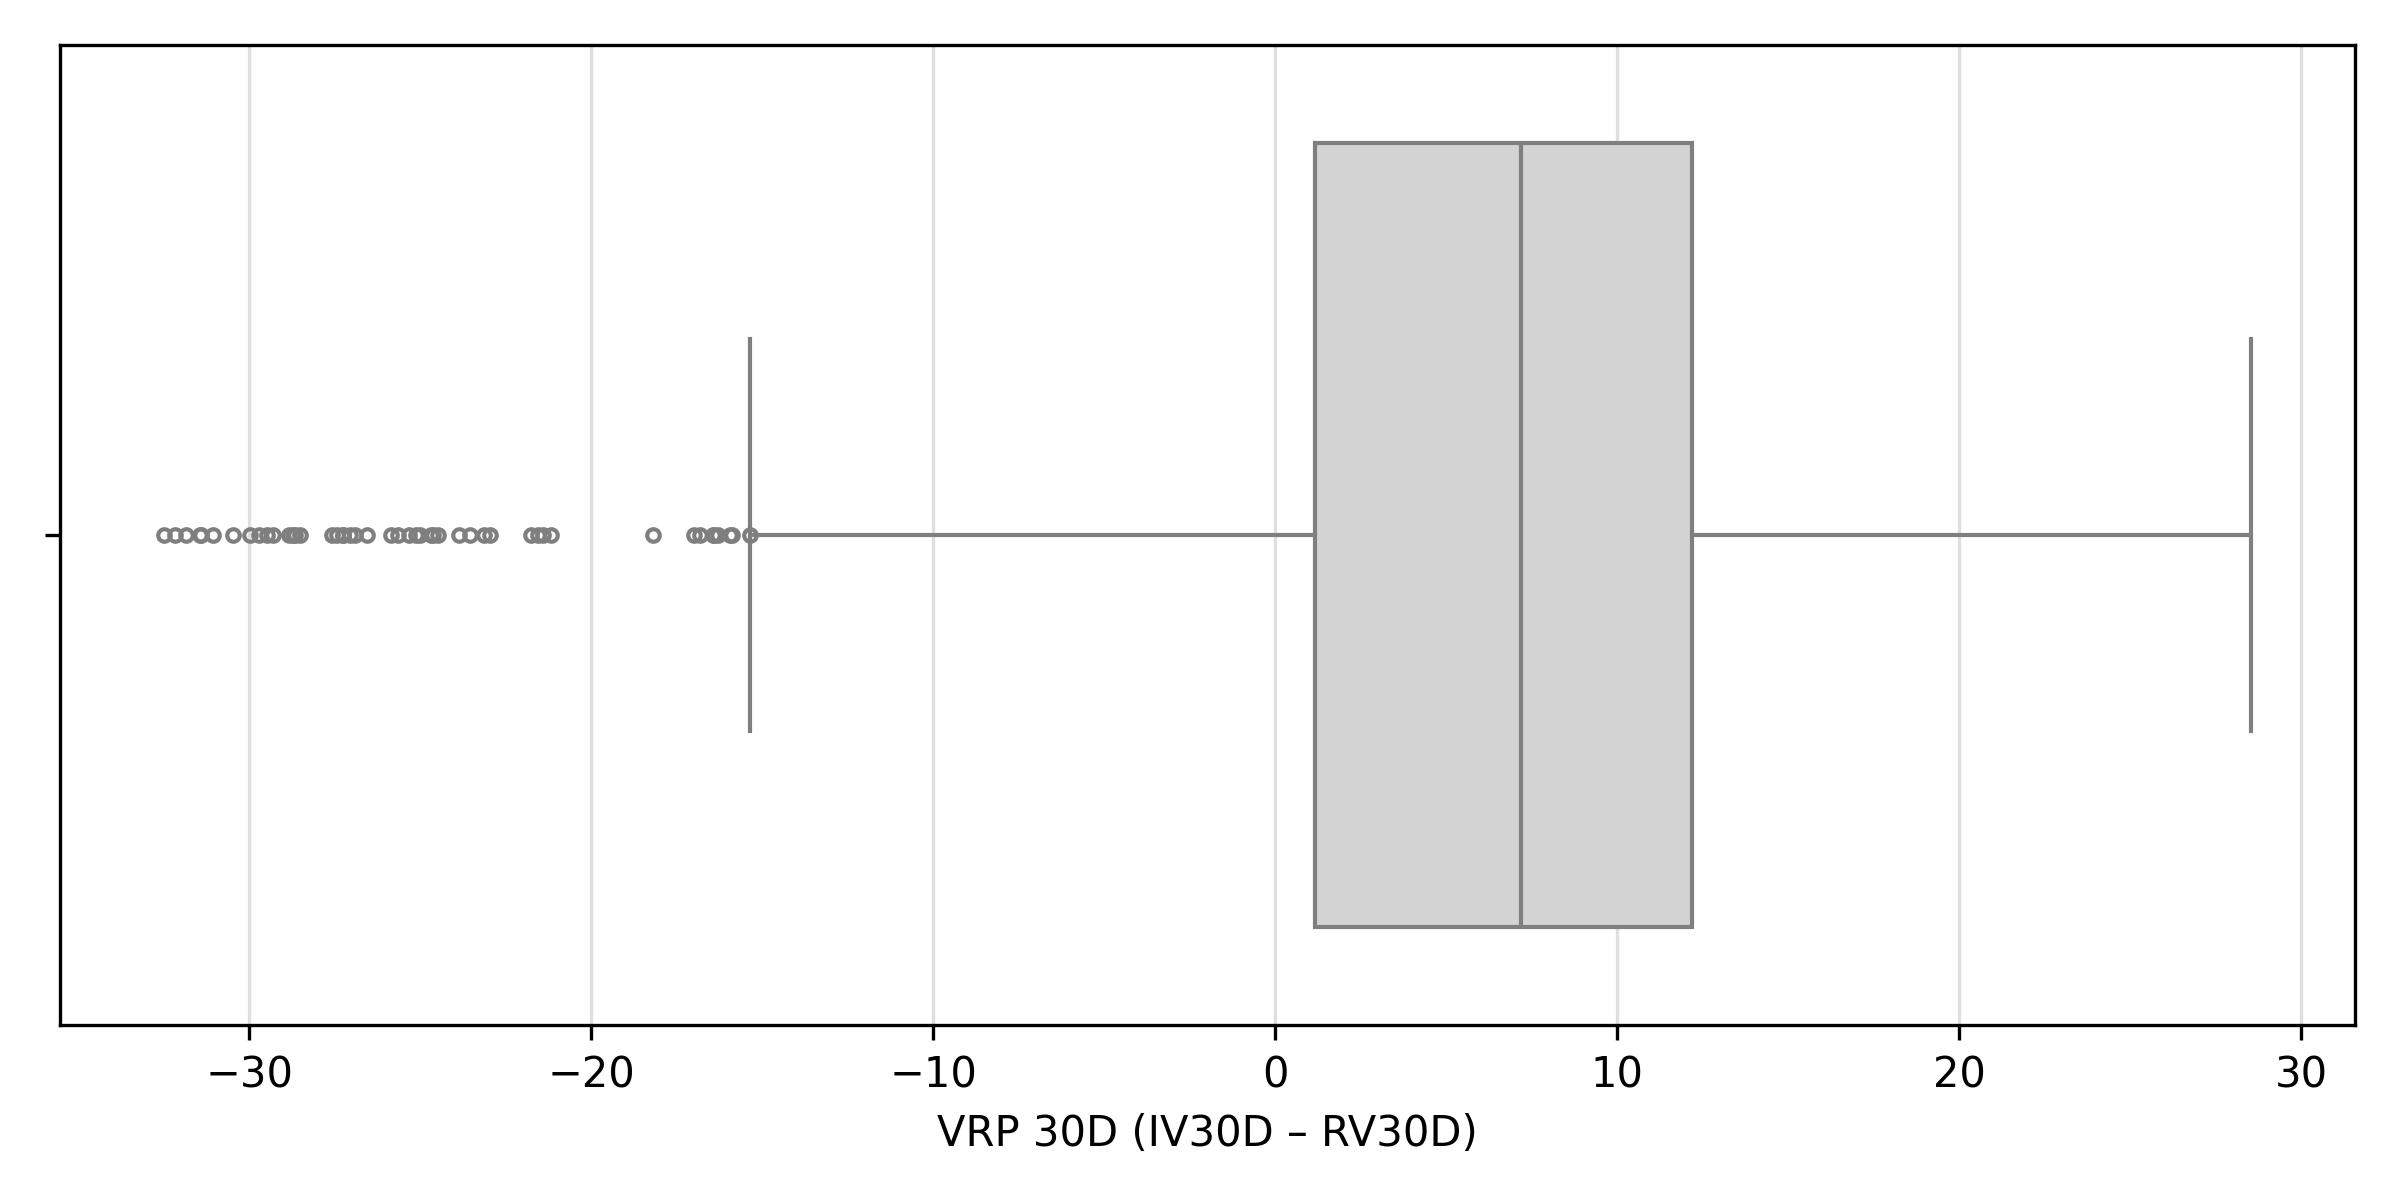
\includegraphics[width=0.92\textwidth]{figs/vrp_boxplot.png}
    \caption{Boxplot geral do VRP ao longo da amostra.}
    \label{fig:vrp_boxplot}
\end{figure}

Observa-se mediana positiva e assimetria negativa pronunciada, com valores
extremos associados a oscilações bruscas de volatilidade.

A Figura~\ref{fig:vrp_boxplot_ano} detalha a distribuição por ano.

\begin{figure}[H]
    \centering
    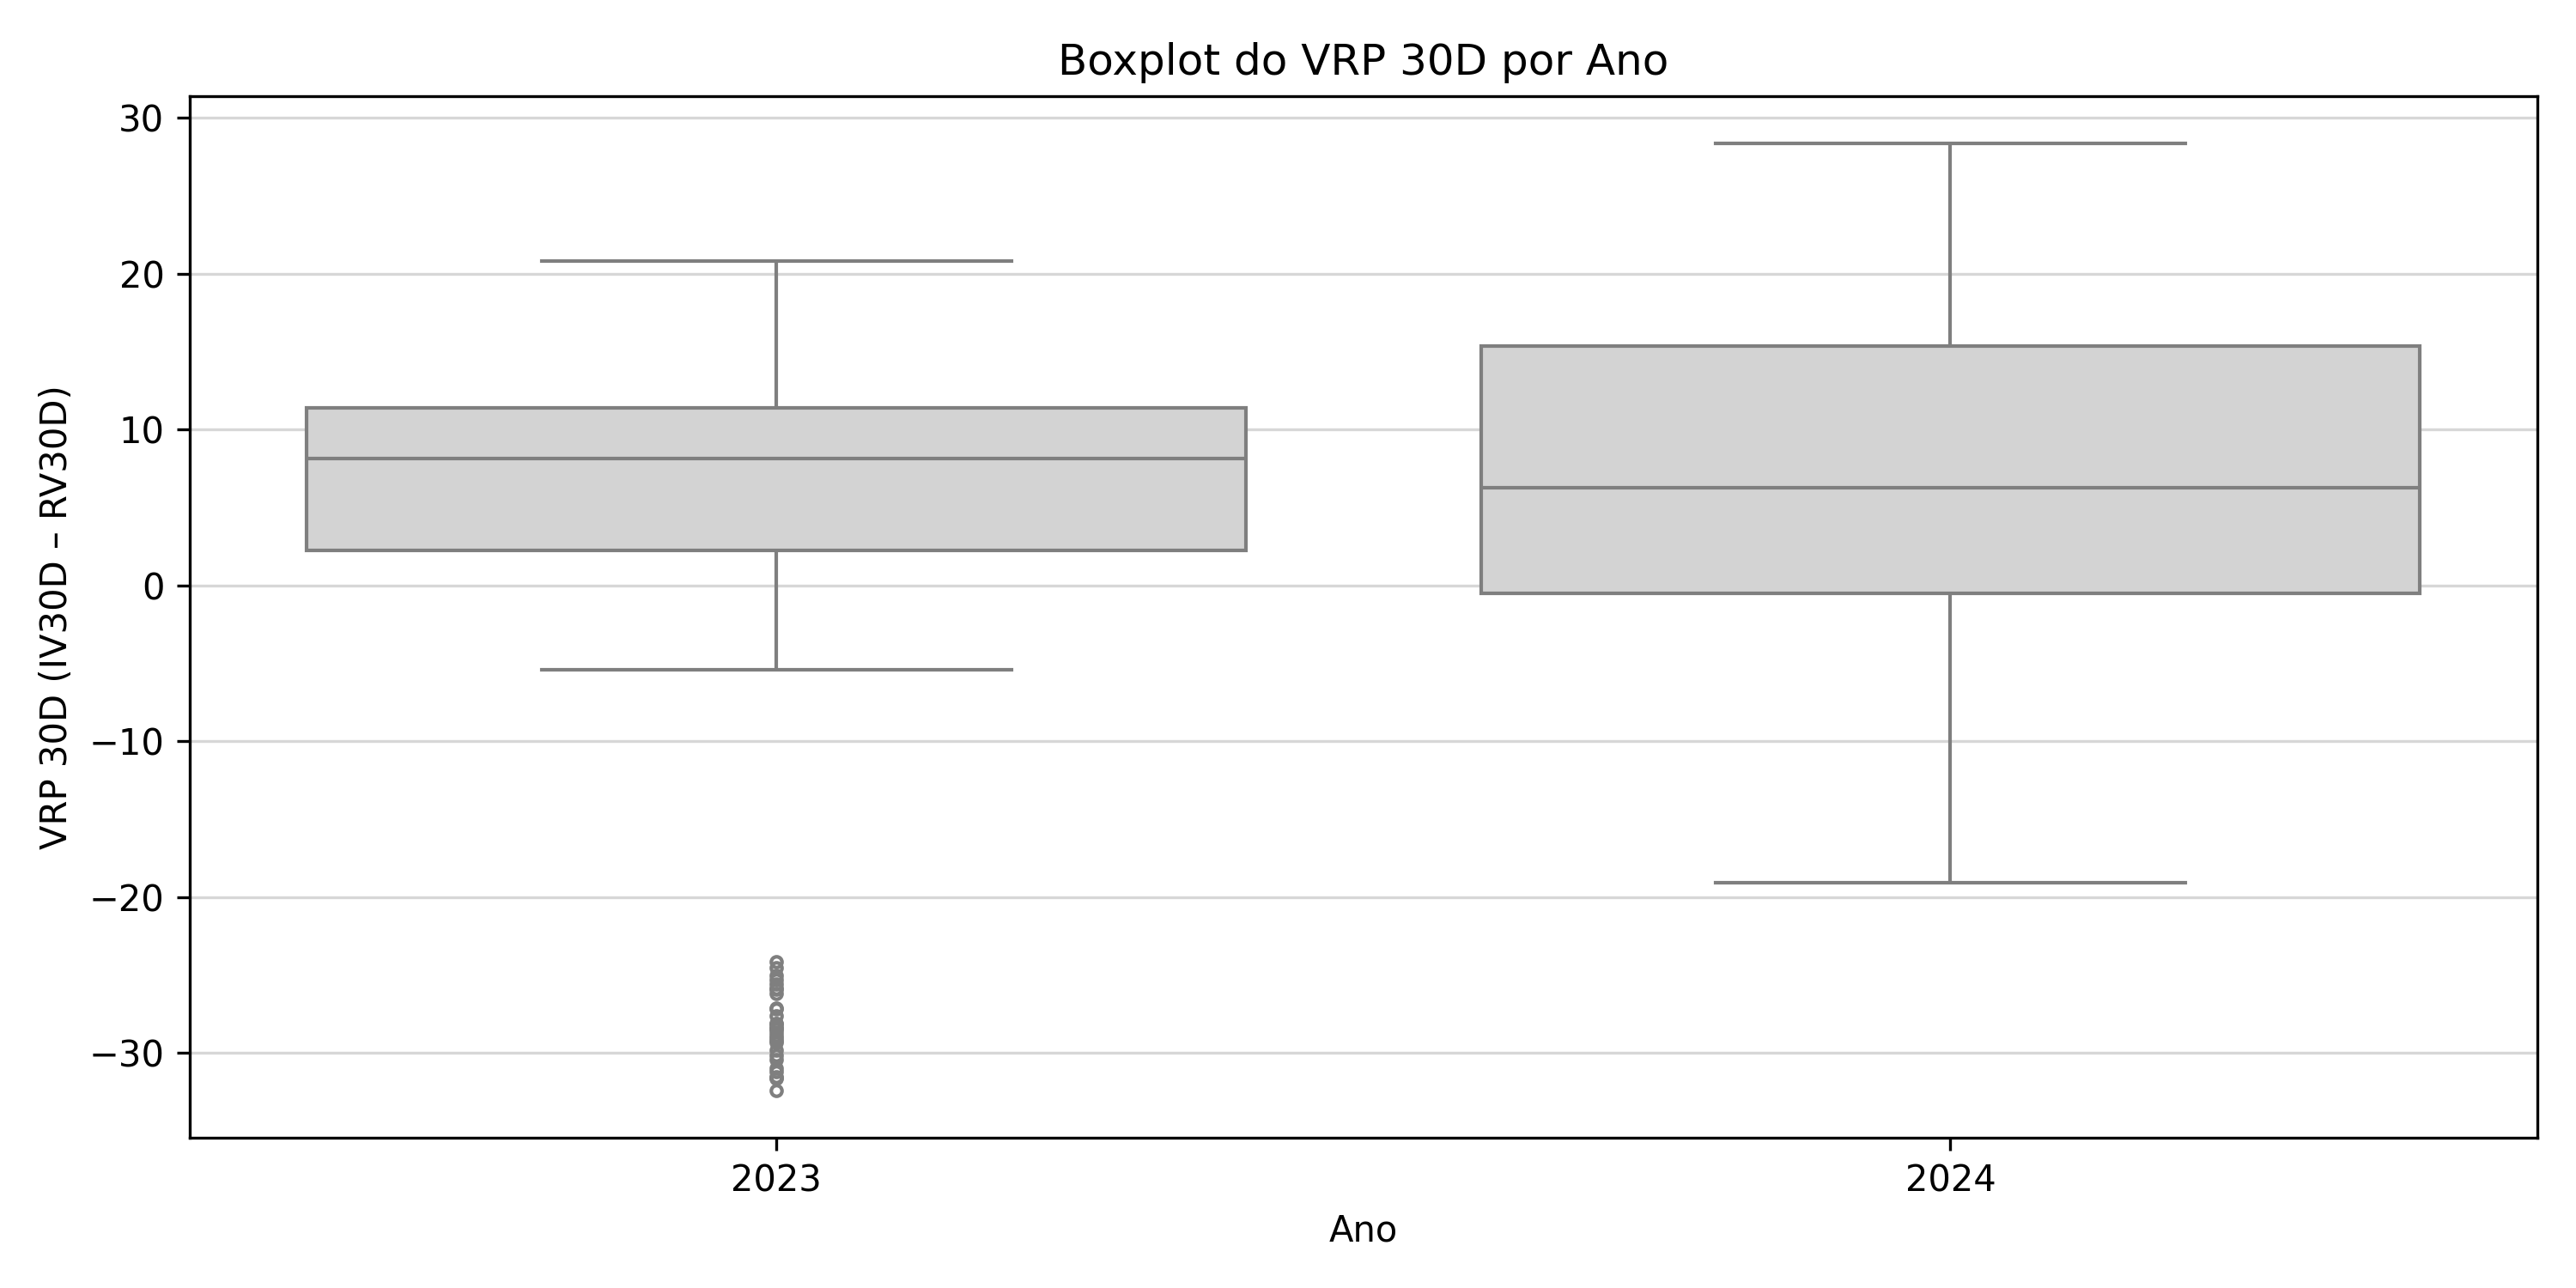
\includegraphics[width=0.92\textwidth]{figs/vrp_boxplot_ano.png}
    \caption{VRP por ano da amostra.}
    \label{fig:vrp_boxplot_ano}
\end{figure}

Os resultados revelam:

\begin{itemize}
    \item anos de maior volatilidade exibem dispersão mais ampla do BVRP;
    \item períodos mais estáveis revelam medianas mais elevadas e menor variação;
    \item mudanças de regime são claramente identificáveis.
\end{itemize}

\section{Relação entre VRP e retornos futuros}

Nesta etapa, são analisadas relações gráficas entre o BVRP e os retornos
futuros do Bitcoin em diferentes horizontes.

\subsection*{Retorno futuro de 1 dia}

\begin{figure}[H]
    \centering
    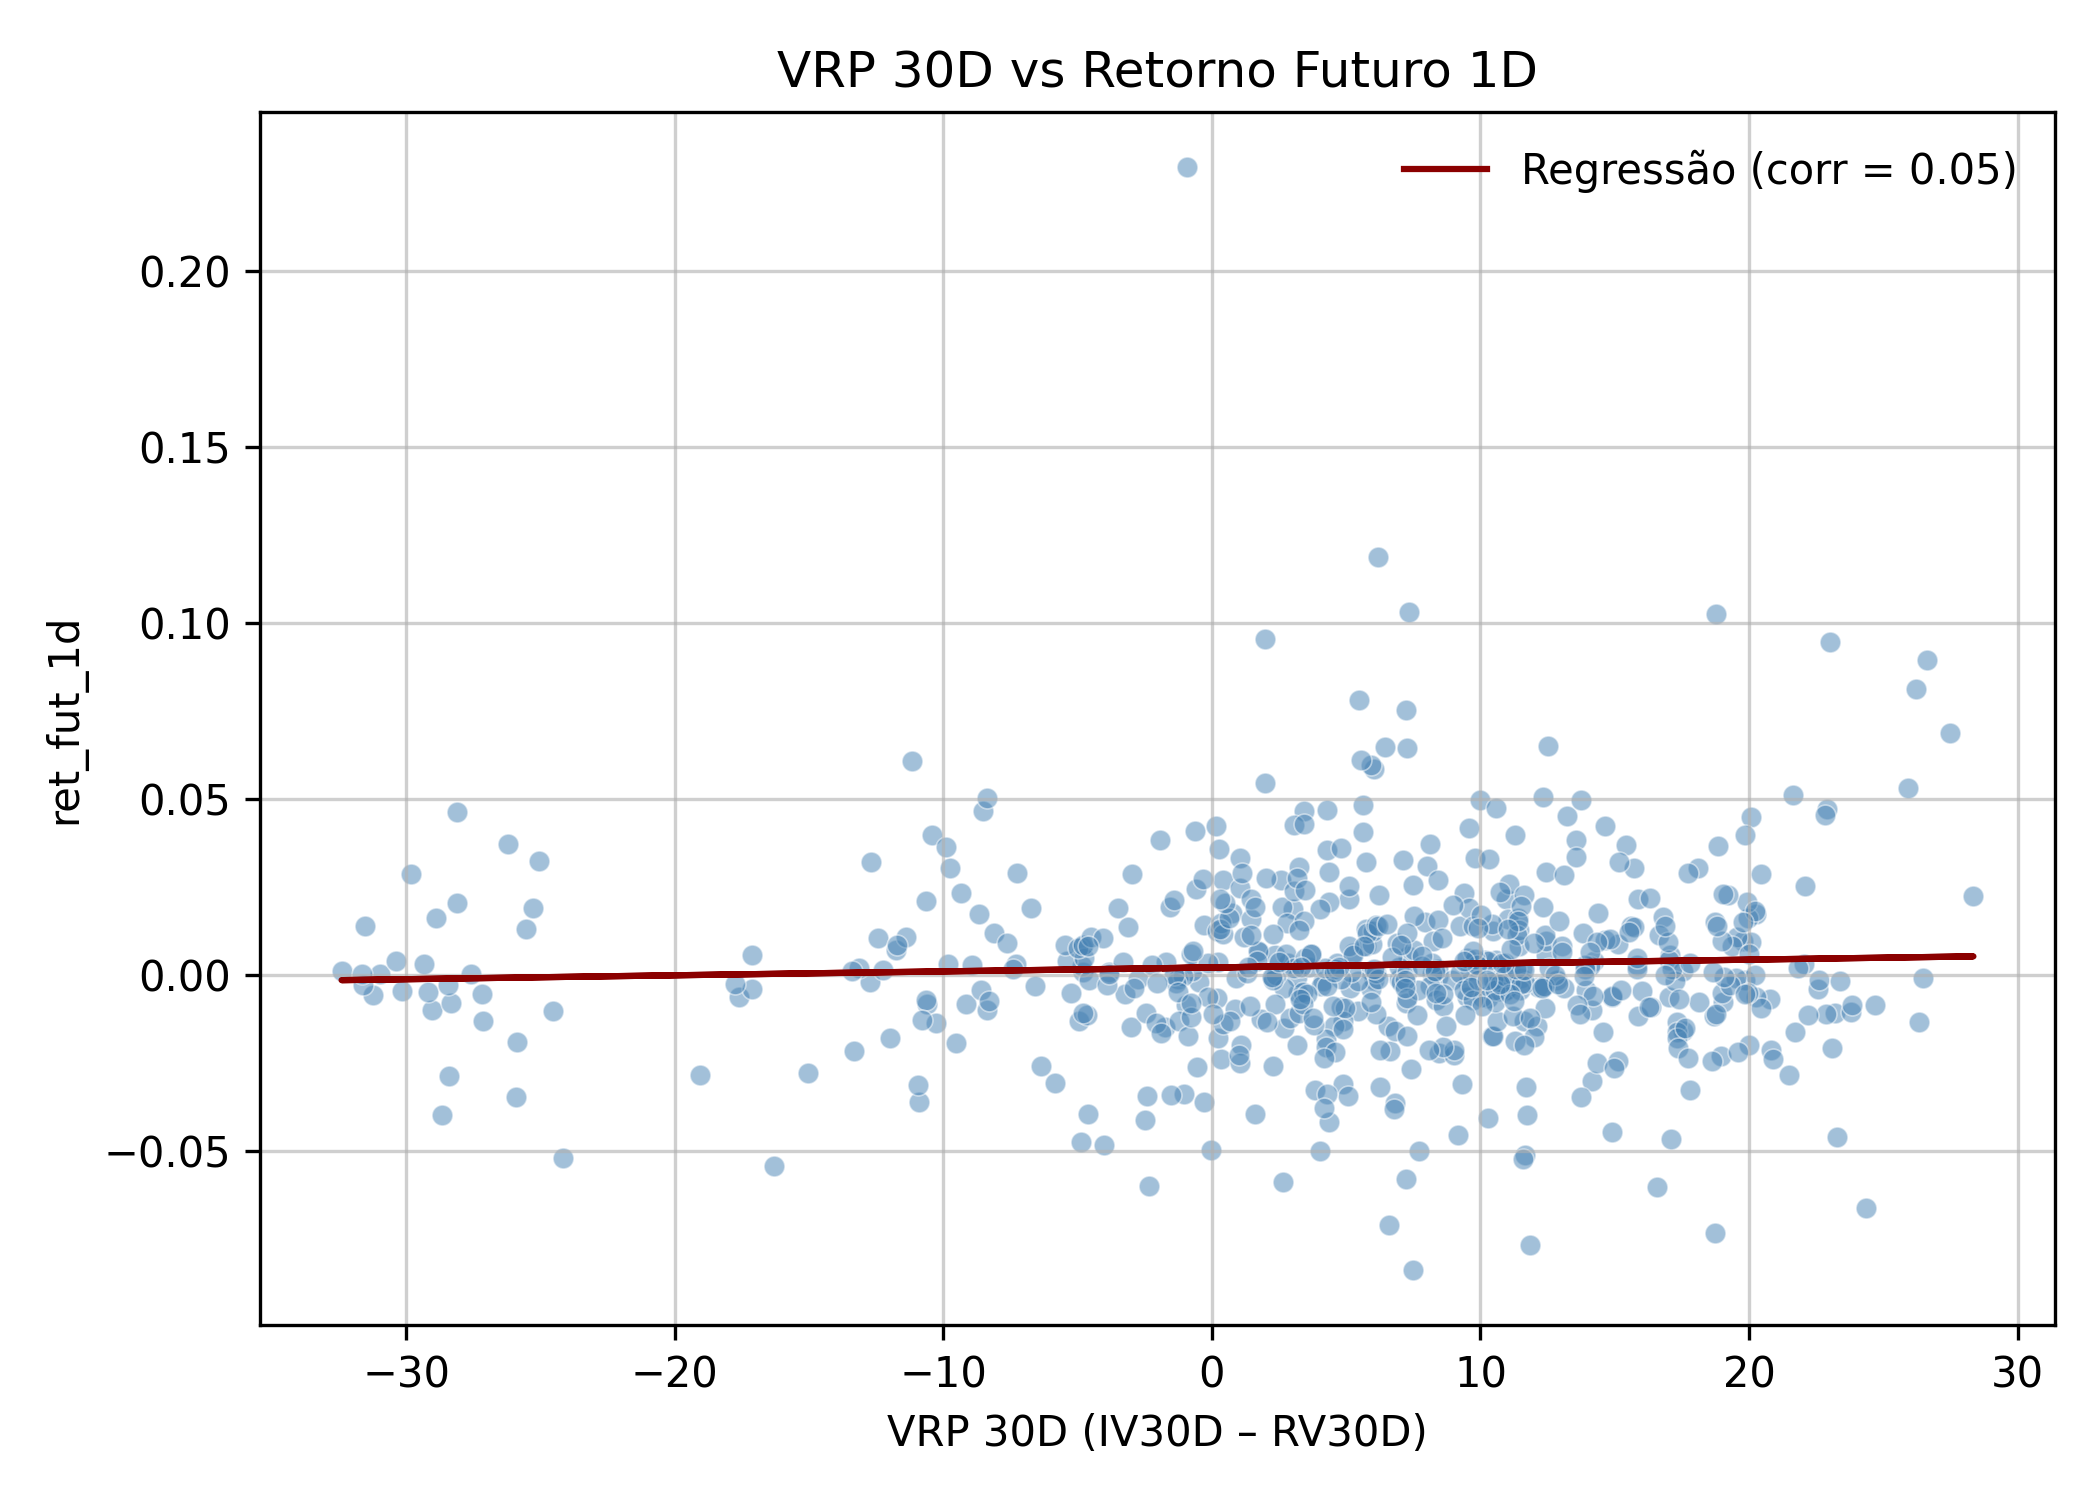
\includegraphics[width=0.9\textwidth]{figs/vrp_vs_return_1d.png}
    \caption{VRP vs. retorno futuro de 1 dia.}
    \label{fig:vrp_vs_ret_1d}
\end{figure}

A relação é fraca e fortemente dispersa, o que é esperado dado que retornos
diários de criptoativos tendem a ser dominados por ruído, microestrutura e
eventos idiossincráticos.

\subsection*{Retorno futuro de 5 dias}

\begin{figure}[H]
    \centering
    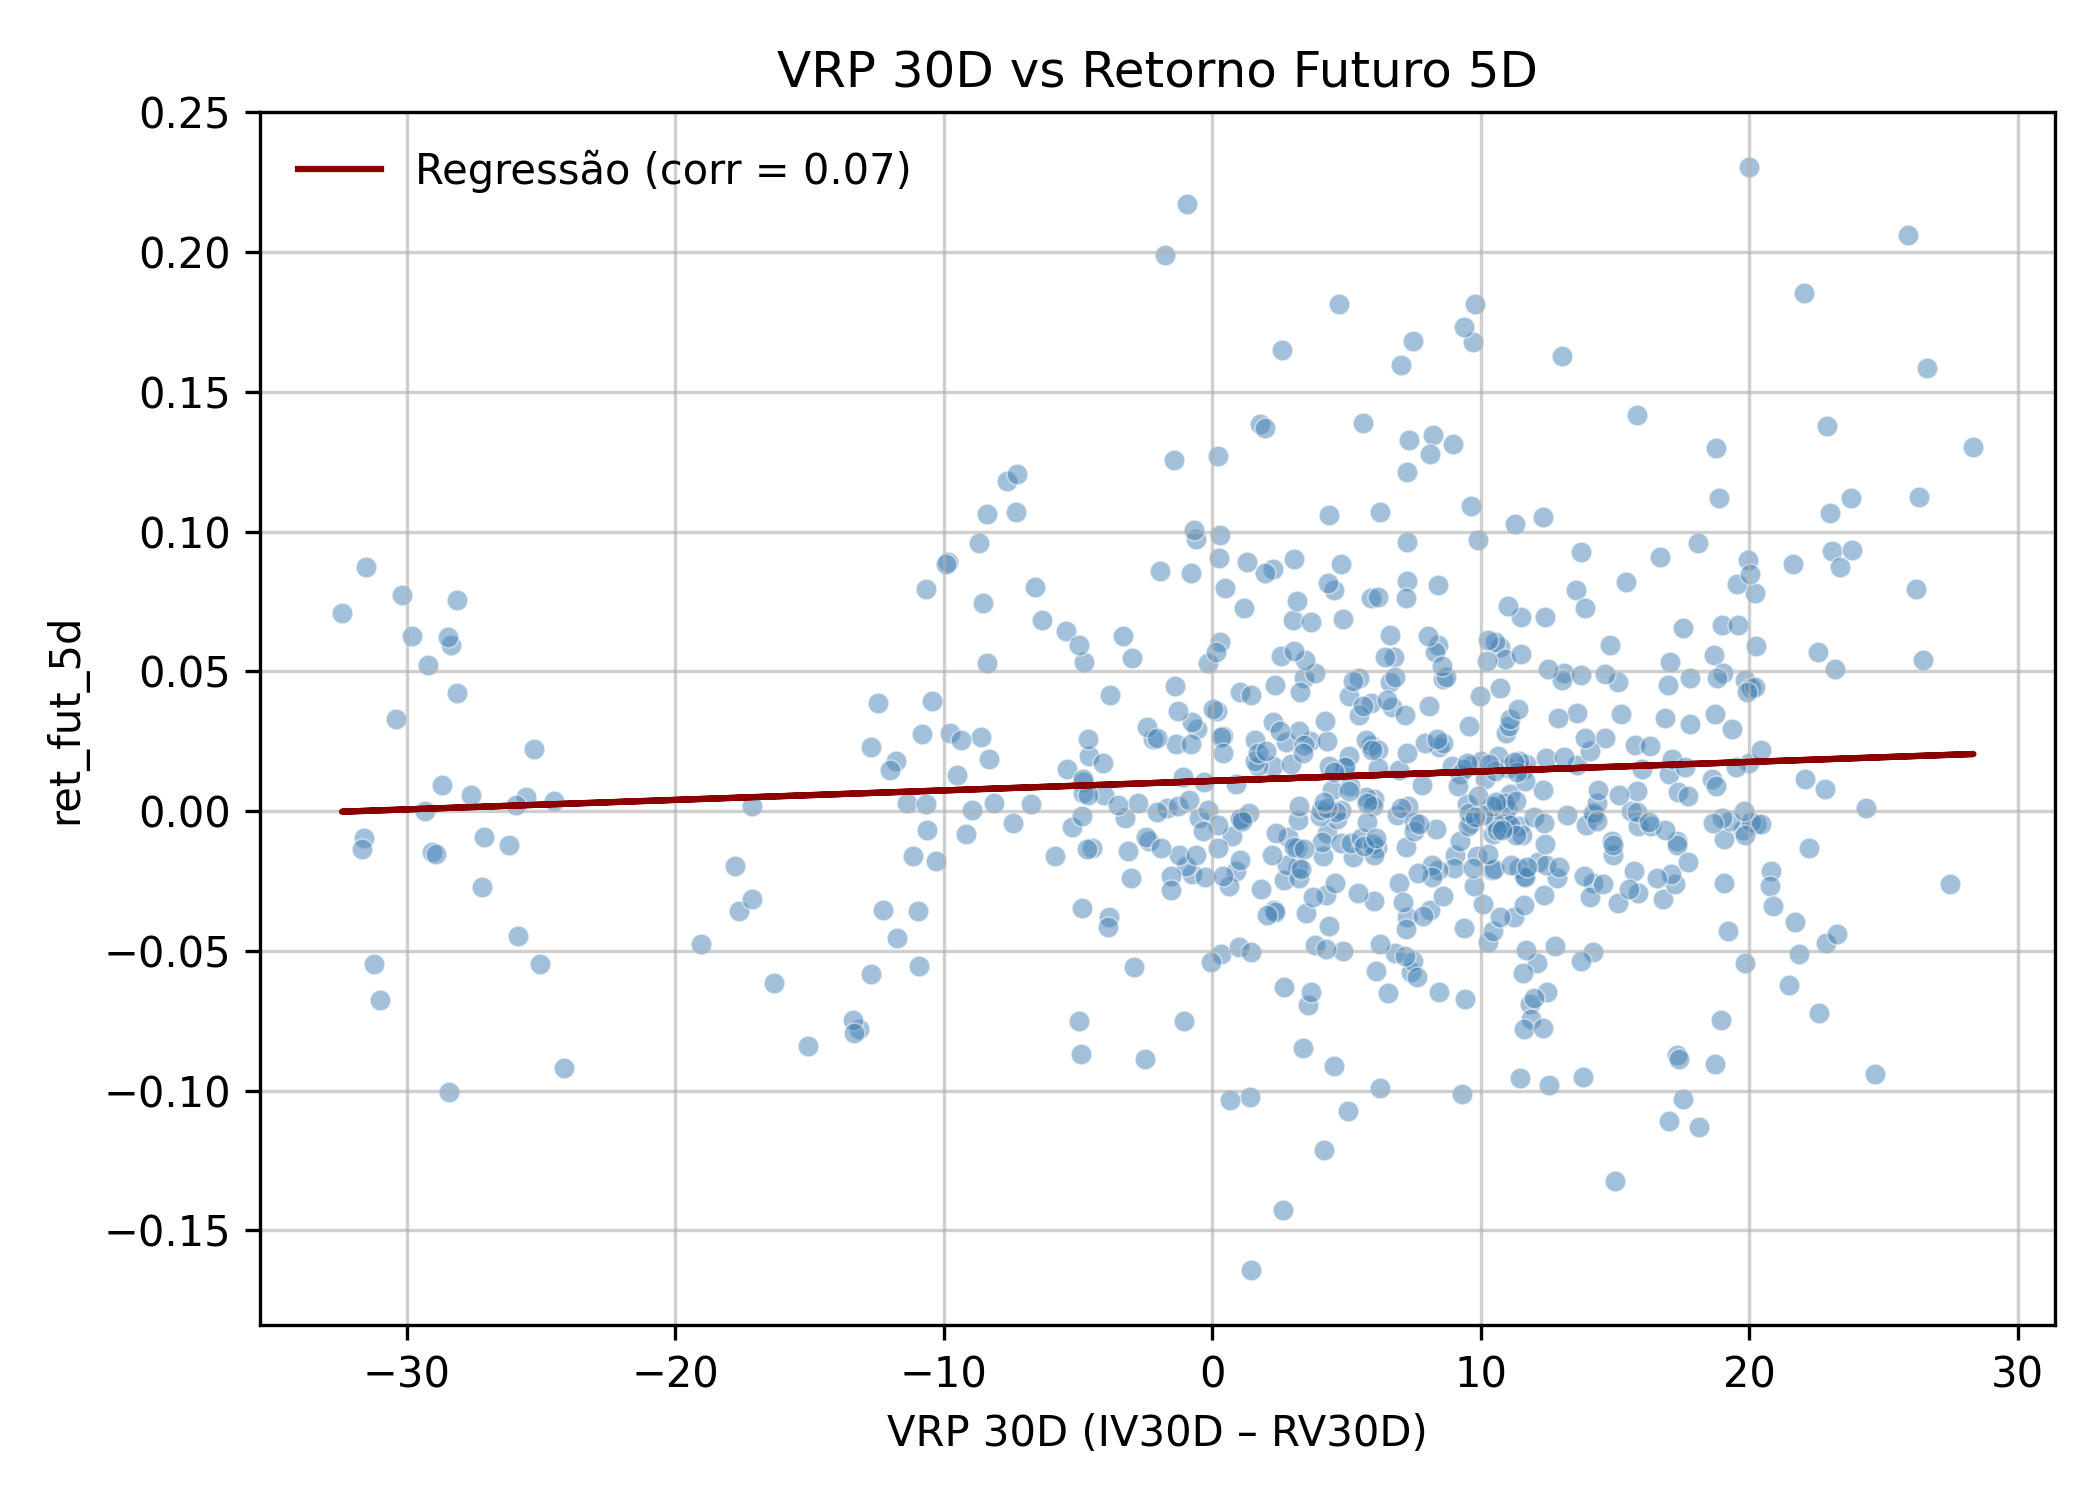
\includegraphics[width=0.9\textwidth]{figs/vrp_vs_return_5d.png}
    \caption{VRP vs. retorno futuro de 5 dias.}
    \label{fig:vrp_vs_ret_5d}
\end{figure}

A inclinação da nuvem de pontos torna-se ligeiramente mais pronunciada,
sugerindo algum grau de previsibilidade em horizontes semanais.

\subsection*{Retorno futuro de 20 dias}

\begin{figure}[H]
    \centering
    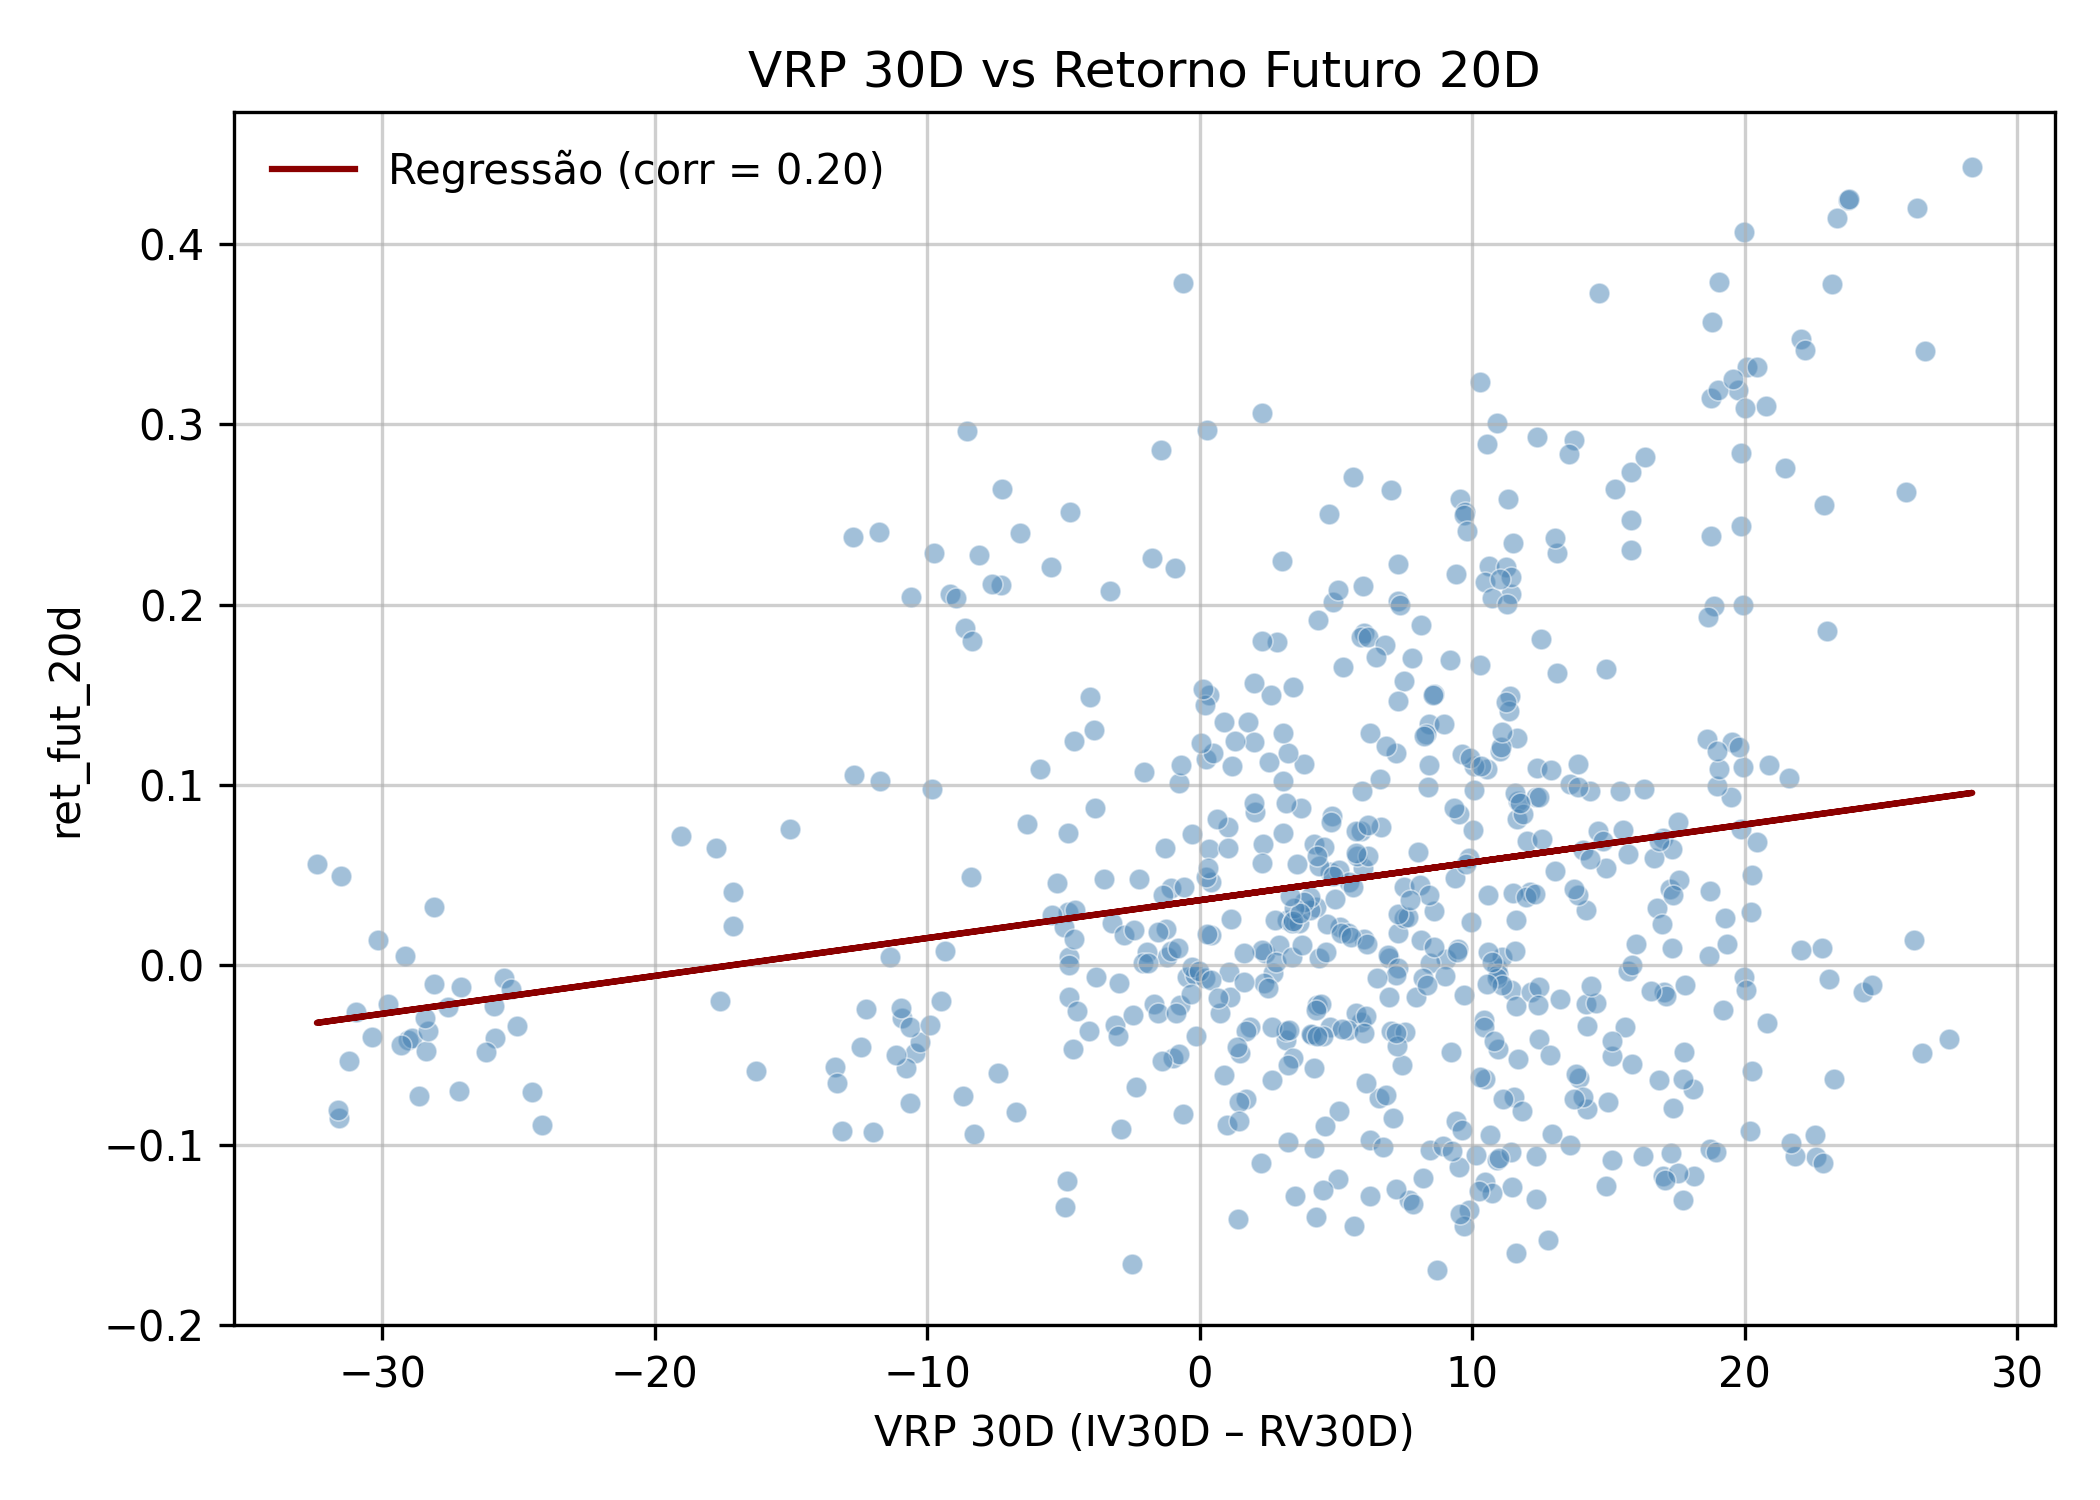
\includegraphics[width=0.9\textwidth]{figs/vrp_vs_return_20d.png}
    \caption{VRP vs. retorno futuro de 20 dias.}
    \label{fig:vrp_vs_ret_20d}
\end{figure}

No horizonte de 20 dias, a relação linear torna-se mais evidente, com maior
concentração dos pontos em torno de uma tendência positiva. Esse resultado
corrobora a hipótese (H4) de que o VRP contém informação preditiva mais clara em
janelas temporais mais longas.

\section{Síntese: o que o VRP nos revela empiricamente}

A partir dos resultados apresentados, é possível sintetizar os seguintes pontos:

\begin{itemize}
    \item O VRP médio é positivo, revelando um prêmio estrutural pago pela
          proteção contra incerteza.
    \item O BVRP apresenta regimes distintos, alternando entre complacência e
          estresse, em linha com a natureza altamente volátil do mercado de
          criptoativos.
    \item A distribuição do BVRP é assimétrica, com cauda inferior pesada,
          refletindo episódios de volatilidade realizada excepcionalmente alta.
    \item A relação com retornos futuros é fraca em horizontes curtos e mais
          clara em horizontes de 20 dias, sugerindo capacidade preditiva
          moderada.
\end{itemize}

\section{Preparação para o capítulo de Machine Learning}

As evidências apresentadas reforçam a necessidade de modelos que capturem
estruturas não lineares e interações complexas entre variáveis. Em particular:

\begin{itemize}
    \item relações não lineares são visíveis nos diagramas de dispersão;
    \item regimes distintos sugerem comportamento segmentado;
    \item variáveis contemporâneas e defasadas interagem de forma não trivial.
\end{itemize}

Essas características motivam o uso de Random Forest e XGBoost, detalhados no
Capítulo~\ref{chap:ml}, onde a análise preditiva é formalizada.


\chapter{Modelos de Machine Learning para Previsão de Retornos}
\label{chap:ml}

Este capítulo apresenta os modelos de aprendizado de máquina utilizados para
avaliar se o \textit{Bitcoin Volatility Risk Premium} (BVRP) contém informação
preditiva relevante para retornos futuros do Bitcoin. A análise concentra-se na
capacidade de modelos não lineares capturarem padrões que métodos lineares
tradicionais não conseguem representar adequadamente, especialmente em um mercado
caracterizado por alta volatilidade, regimes distintos e forte presença de ruído.

Foram considerados dois algoritmos amplamente utilizados em finanças
quantitativas: \textit{Random Forest} e \textit{XGBoost}, ambos baseados em
estruturas de árvores, porém com mecanismos distintos de agregação e ajuste.

\section{Estrutura geral dos modelos}

Os modelos foram treinados com um conjunto ampliado de variáveis explicativas que
capturam tanto características contemporâneas quanto defasadas do mercado. Entre
elas:

\begin{itemize}
    \item BVRP (IV30D -- RV30D);
    \item IV30D e RV30D individualmente;
    \item medidas adicionais de volatilidade realizada (RV7D, RV14D);
    \item retornos passados do Bitcoin (1D, 3D, 5D);
    \item lags das variáveis principais (1 a 3 dias);
    \item indicadores de tendência (retornos acumulados);
    \item dummies de regime quando aplicável (IV alta vs. IV baixa).
\end{itemize}

O alvo principal escolhido para esta etapa é o retorno futuro de 5 dias
(\textit{ret\_fut\_5d}), identificado no Capítulo~\ref{chap:analise_empirica}
como o horizonte com maior relação empírica com o BVRP sem perda excessiva de
amostra.

\section{Random Forest}

O Random Forest é um método baseado em \textit{bagging}, no qual múltiplas
árvores de decisão são estimadas a partir de amostras bootstrap dos dados.
Suas vantagens incluem robustez a outliers, capacidade de modelar relações não
lineares e menor risco de overfitting quando comparado a árvores individuais.

A Figura~\ref{fig:rf_ret5d} apresenta os valores reais versus previstos para o
retorno futuro de 5 dias.

\begin{figure}[H]
    \centering
    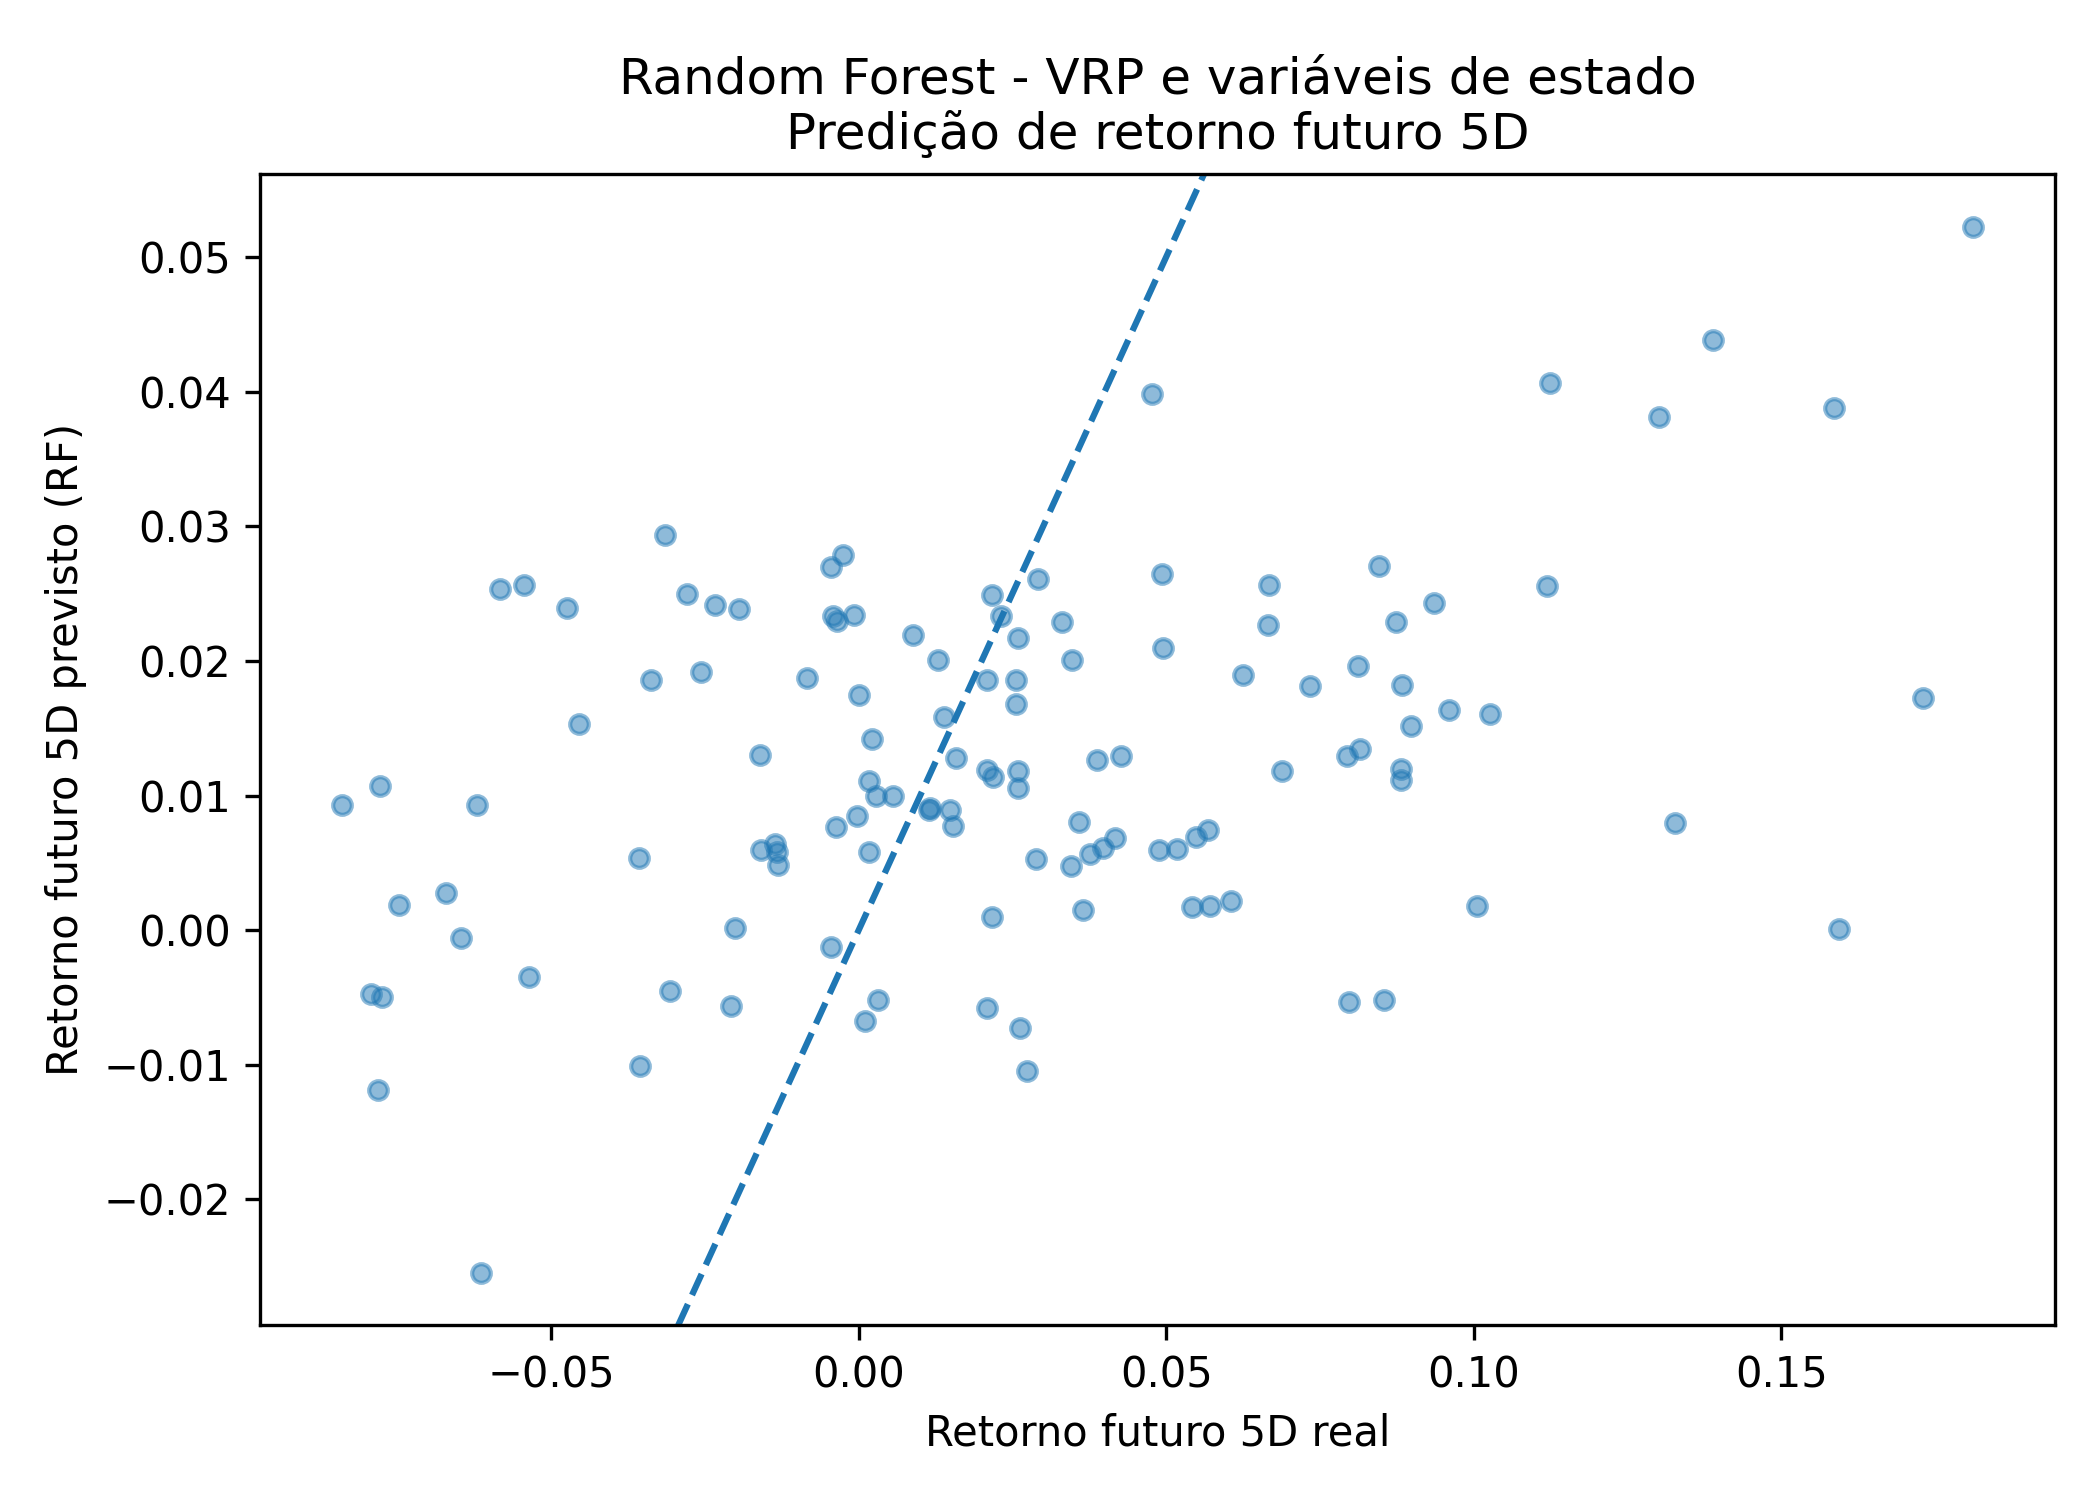
\includegraphics[width=0.9\textwidth]{figs/rf_ret_fut_5d_real_vs_pred.png}
    \caption{Random Forest: valores reais versus previstos para o retorno futuro de 5 dias.}
    \label{fig:rf_ret5d}
\end{figure}

O modelo apresenta capacidade limitada, mas não desprezível, de capturar a
direção dos movimentos, embora tenda a suavizar as previsões — comportamento
típico de modelos de árvore agregados.

\section{XGBoost}

O XGBoost emprega uma estratégia de \textit{gradient boosting}, em que árvores
são adicionadas sequencialmente para corrigir os resíduos dos modelos anteriores.
A presença de regularização explícita (L1 e L2) e mecanismos de controle de
complexidade tornam o algoritmo particularmente adequado para detectar padrões
sutis em séries financeiras ruidosas.

A Figura~\ref{fig:xgb_ret5d} apresenta a comparação entre valores reais e previstos
pelo XGBoost.

\begin{figure}[H]
    \centering
    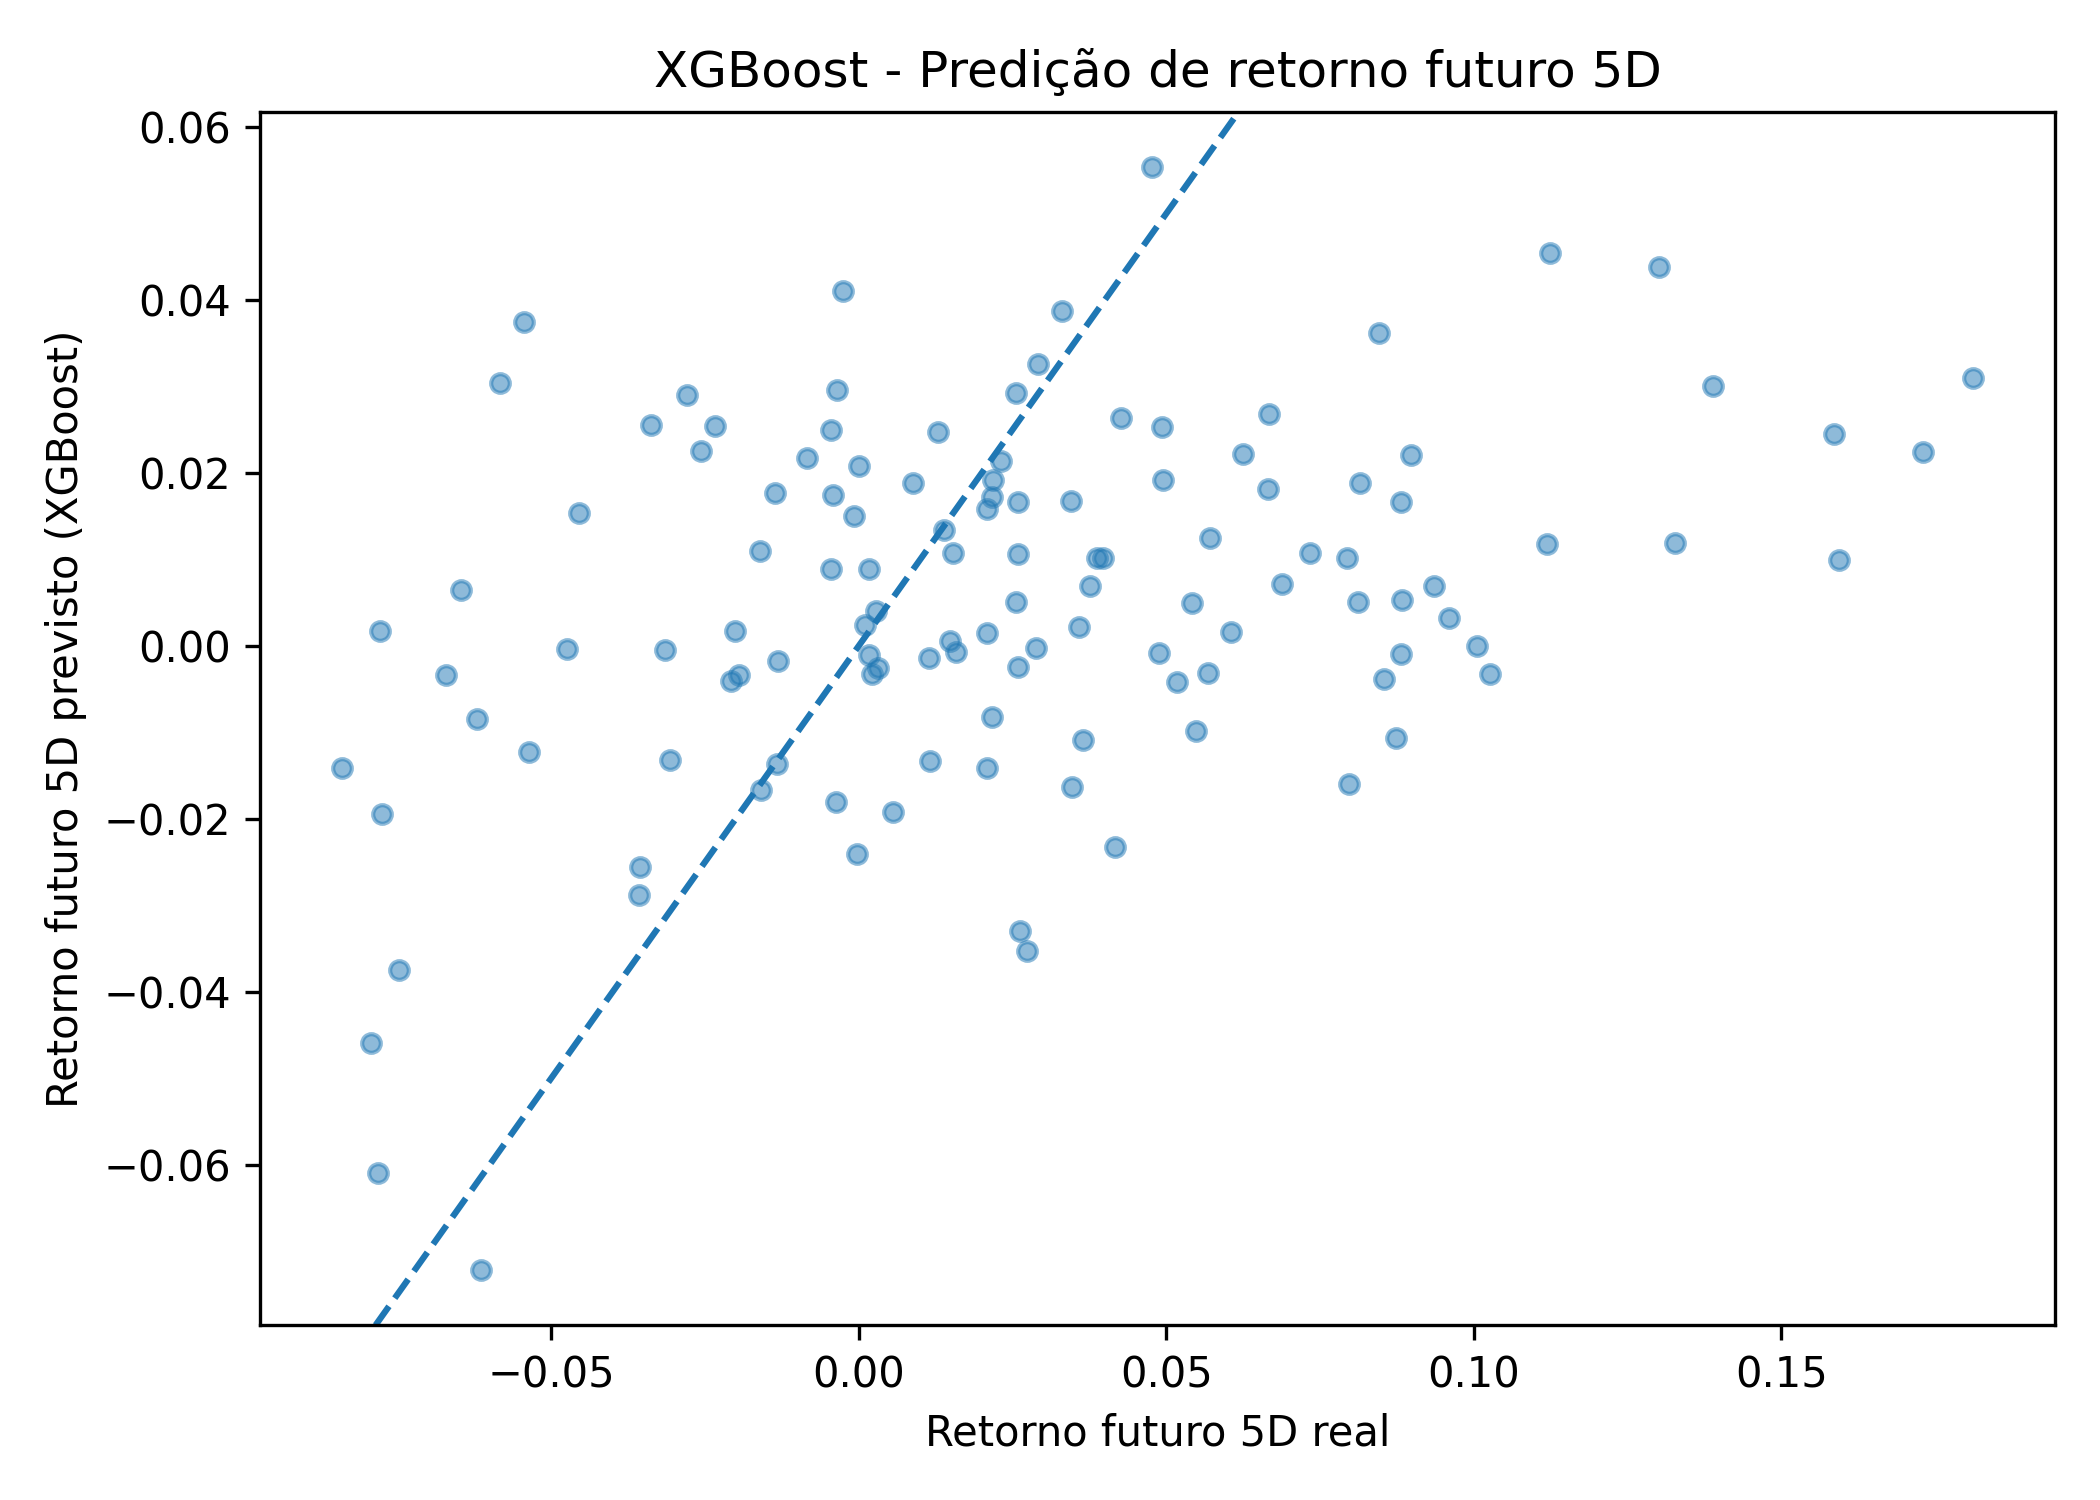
\includegraphics[width=0.9\textwidth]{figs/xgb_ret_fut_5d_real_vs_pred.png}
    \caption{XGBoost: valores reais versus previstos para o retorno futuro de 5 dias.}
    \label{fig:xgb_ret5d}
\end{figure}

O modelo exibe melhor aderência em relação ao Random Forest, embora continue
enfrentando dificuldade para capturar movimentos extremos — padrão amplamente
documentado na literatura sobre previsão de retornos em mercados altamente
voláteis.

\section{Comparação entre os modelos}

A comparação dos modelos indica:

\begin{itemize}
    \item ambos apresentam correlação positiva entre valores reais e previstos;
    \item o XGBoost obtém menor erro médio (MAE e MSE) e melhor alinhamento visual;
    \item o BVRP contribui marginalmente para o ajuste, embora seu efeito isolado
          permaneça limitado;
    \item a previsibilidade melhora conforme o horizonte de retorno aumenta,
          especialmente para 20 dias, em linha com a análise do capítulo anterior.
\end{itemize}

Essas evidências reforçam que o VRP carrega informação, mas em magnitude moderada,
e que modelos não lineares são mais eficazes para extraí-la.

\section{Importância das variáveis}

A análise de importância (feature importance) revela que:

\begin{enumerate}
    \item a volatilidade realizada (RV30D) é a variável mais relevante;
    \item o BVRP possui importância consistente, especialmente no XGBoost;
    \item retornos passados auxiliam na estabilização do ruído;
    \item a IV30D apresenta efeito dependente de regime (mais útil em momentos de
          incerteza elevada).
\end{enumerate}

Esses resultados estão alinhados com estudos anteriores que destacam o papel
dominante da volatilidade na estrutura de retornos de ativos de alto risco.

\section{Limitações}

Ainda que os resultados sejam consistentes, algumas limitações devem ser
consideradas:

\begin{itemize}
    \item previsões de retornos em criptoativos permanecem altamente ruidosas;
    \item modelos de árvore têm dificuldade com movimentos extremos;
    \item tuning mais profundo poderia melhorar métricas, mas aumentaria risco de
          overfitting;
    \item previsibilidade estatística não implica necessariamente lucratividade
          após custos de transação.
\end{itemize}

\section{Síntese}

Os modelos Random Forest e XGBoost sugerem que:

\begin{itemize}
    \item o BVRP contém informação incremental para previsão de retornos;
    \item essa informação se manifesta principalmente em horizontes mais longos;
    \item modelos não lineares capturam parcialmente essa relação;
    \item a capacidade preditiva permanece moderada, em linha com a literatura de
          finanças de alta volatilidade.
\end{itemize}

O próximo capítulo integra esses achados a uma discussão operacional, abordando
implicações práticas e limitações para uso do BVRP em estratégias quantitativas.

\chapter{Implicações Operacionais e Estratégias Baseadas no BVRP}
\label{chap:estrategias}

Este capítulo integra os resultados empíricos e preditivos apresentados ao longo
da dissertação e discute como o \textit{Bitcoin Volatility Risk Premium} (BVRP)
pode ser utilizado de forma prática em estratégias quantitativas, gestão de
risco, monitoramento de regimes e alocação tática. São avaliadas oportunidades,
limitações e cuidados necessários no uso de volatilidade implícita e realizada em
uma classe de ativos caracterizada por forte assimetria, regimes distintos e
alta frequência de eventos extremos.

\section{O BVRP como indicador de regime de mercado}

Os resultados dos capítulos anteriores sugerem que o BVRP apresenta dinâmicas
claras que refletem diferentes estados do mercado de Bitcoin. Três regimes
podem ser identificados de maneira recorrente:

\begin{itemize}
    \item \textbf{Regime de complacência (BVRP elevado e positivo):}  
          a volatilidade implícita permanece acima da realizada, sinalizando
          demanda consistente por proteção ou expectativas de tranquilidade.
    \item \textbf{Regime de estresse (BVRP negativo):}  
          a volatilidade realizada ultrapassa a implícita de forma abrupta, em
          geral associada a liquidações, picos de incerteza ou choques idiossincráticos.
    \item \textbf{Regime de transição (BVRP crescente ou declinante):}  
          o mercado ajusta gradualmente sua percepção de risco, antecipando
          mudanças de volatilidade futura.
\end{itemize}

Esses regimes possuem interpretações operacionais relevantes:

\begin{itemize}
    \item BVRP elevado tende a coincidir com períodos de estabilização de volatilidade;
    \item BVRP negativo está frequentemente associado a reversões de curto prazo;
    \item BVRP crescente indica intensificação de incerteza e aproximação de eventos relevantes.
\end{itemize}

Assim, o BVRP funciona como um indicador \emph{útil}, embora não suficiente,
para caracterizar condições de mercado e modular exposições em estratégias
quantitativas.

\section{Estratégias baseadas em volatilidade}

A literatura financeira documenta amplamente que o VRP pode oferecer
oportunidades operacionais quando a volatilidade implícita tende a exceder a
volatilidade realizada. Para Bitcoin, duas categorias principais de estratégias
são aplicáveis.

\subsection{Venda sistemática de volatilidade implícita}

Em períodos de BVRP elevado, estratégias que vendem volatilidade se tornam
naturalmente atrativas. Entre as estruturas possíveis:

\begin{itemize}
    \item \textit{short strangles} e \textit{short straddles} (com hedge de delta);
    \item estruturas de \textit{iron condor};
    \item venda de volatilidade via contratos perpétuos com hedge direcional.
\end{itemize}

\textbf{Riscos principais:}

\begin{itemize}
    \item movimentos extremos e unidirecionais (\textit{short gamma risk});
    \item liquidações em cascata típicas do mercado de cripto;
    \item custo operacional elevado de hedges dinâmicos.
\end{itemize}

\subsection{Compra de volatilidade realizada (BVRP negativo)}

Quando o BVRP é negativo, a volatilidade realizada supera a implícita, abrindo
espaço para estratégias compradas em volatilidade, tais como:

\begin{itemize}
    \item compra de \textit{straddles} para capturar movimentos abruptos;
    \item estruturas delta-neutras focadas em eventos de estresse;
    \item compra direcional de opções fora-do-dinheiro em períodos de queda.
\end{itemize}

Essas abordagens são consistentes com literatura que documenta o caráter
reversivo da volatilidade realizada em eventos extremos.

\section{Estratégias direcionais baseadas no BVRP}

Ainda que o BVRP seja uma medida de volatilidade, sua relação com retornos pode
ser explorada de forma direcional. Os resultados empíricos sugerem:

\begin{itemize}
    \item \textbf{BVRP alto} tende a ocorrer em mercados mais estáveis, com retornos
          moderadamente positivos;
    \item \textbf{BVRP baixo} indica assimetria negativa e maior incerteza;
    \item \textbf{BVRP negativo} frequentemente coincide com reversões e movimentos
          de estresse.
\end{itemize}

No Capítulo~\ref{chap:ml}, observou-se que:

\begin{itemize}
    \item existe relação preditiva, principalmente em horizontes de 20 dias;
    \item o sinal é estatisticamente relevante, mas moderado;
    \item o BVRP não deve ser usado como gatilho isolado para entrada.
\end{itemize}

Assim, o uso mais adequado é como \textbf{filtro de condições de mercado} em
sistemas quantitativos.

\section{Integração do BVRP em modelos quantitativos}

A integração do BVRP com estratégias quantitativas pode ocorrer de diversas
formas.

\subsection{Filtros de volatilidade}

\begin{itemize}
    \item permitir operações apenas quando o BVRP estiver acima/abaixo de limites;
    \item ajustar tamanhos de posição conforme a magnitude do BVRP;
    \item identificar transições de regime para modular exposição.
\end{itemize}

\subsection{Sinais compostos}

O BVRP pode complementar outros indicadores:

\begin{itemize}
    \item medidas de momentum;
    \item indicadores de fluxo de opções (put/call ratio, volume implícito);
    \item \textit{funding rates} de futuros perpétuos;
    \item spreads spot–perpétuo.
\end{itemize}

\subsection{Modelos híbridos com Machine Learning}

Os modelos Random Forest e XGBoost demonstraram que:

\begin{itemize}
    \item o BVRP possui importância moderada como variável explicativa;
    \item combinações de volatilidade + retornos passados melhoram previsões;
    \item padrões não lineares são significativos na relação entre variáveis.
\end{itemize}

Esses resultados sugerem que o BVRP é mais útil como \emph{input} incremental
dentro de modelos mais abrangentes.

\section{Limitações práticas}

Apesar das oportunidades, o uso do BVRP em estratégias operacionais enfrenta
limitações importantes:

\begin{itemize}
    \item custos de transação elevados e \textit{slippage} na Deribit;
    \item risco de liquidações automáticas em posições alavancadas;
    \item descontinuidade parcial de liquidez em horários específicos;
    \item regime 24/7, exigindo monitoramento constante;
    \item sensibilidade a eventos inesperados (\textit{exchange hacks},
          anúncios regulatórios, quedas de infraestrutura).
\end{itemize}

Além disso, operar volatilidade implica lidar com assimetria de risco,
especialmente para estratégias vendidas.

\section{Conclusões integradas}

Os resultados desta dissertação permitem sintetizar:

\begin{itemize}
    \item o BVRP é positivo em média, refletindo prêmio estrutural por proteção;
    \item apresenta regimes claros e assimetria estatística;
    \item carrega informação preditiva moderada, especialmente em horizontes mais longos;
    \item modelos não lineares capturam essa informação melhor que modelos lineares;
    \item o BVRP é mais eficaz como indicador de regime do que como sinal isolado de entrada.
\end{itemize}

\section{Sugestões de extensões futuras}

Possíveis caminhos para aprofundar o estudo incluem:

\begin{itemize}
    \item modelagem explícita via \textit{Markov Switching};
    \item incorporação de dados do livro de ordens (order book);
    \item uso de volatilidade intradiária (\textit{realized volatility HF});
    \item extensão para ETH e outros ativos com mercado de opções líquido;
    \item utilização de modelos de séries temporais com memória longa e redes
          neurais recorrentes (LSTM/GRU).
\end{itemize}

Essas extensões podem aprimorar a compreensão da dinâmica do VRP em cripto e
seu papel em estratégias quantitativas.

\appendix
